\documentclass{amsart}
\usepackage{amsmath,amssymb,amsthm,color,enumerate,latexsym}
\usepackage[bookmarks=true,colorlinks=true, linkcolor=blue, citecolor=cyan]{hyperref}
\usepackage[margin=1in]{geometry}
\usepackage{tikz}
\usepackage{pgflibraryarrows}
\usepackage{pgflibrarysnakes}

\newtheorem{theorem}{Theorem}[section]
\newtheorem*{maintheorem}{Main Theorem}
\newtheorem{algorithm}[theorem]{Algorithm}
\newtheorem{claim}[theorem]{Claim}
\newtheorem{conjecture}[theorem]{Conjecture}
\newtheorem{corollary}[theorem]{Corollary}
\newtheorem{definition}[theorem]{Definition}
\newtheorem{example}[theorem]{Example}
\newtheorem{lemma}[theorem]{Lemma}
\newtheorem{sublemma}{Lemma}[theorem]
\newtheorem{proposition}[theorem]{Proposition}
\newtheorem{remark}[theorem]{Remark}
\newtheorem*{remark*}{Remark}


\newcommand{\bfa}{\mathbf{a}}
\newcommand{\cC}{\mathcal{C}}
\newcommand{\cD}{\mathcal{D}}
\newcommand{\cF}{\mathcal{F}}
\newcommand{\cG}{\mathcal{G}}
\newcommand{\cL}{\mathcal{L}}
\newcommand{\FF}{\mathbb{F}}
\newcommand{\kk}{\Bbbk}
\renewcommand{\AA}{\mathbb{A}}
\newcommand{\CC}{\mathbb{C}}
\newcommand{\KK}{\mathbb{K}}
\newcommand{\RR}{\mathbb{R}}
\newcommand{\ZZ}{\mathbb{Z}}


\newcommand{\supp}{\operatorname{supp}}
\newcommand{\lsh}{\operatorname{lsh}}
\newcommand{\Arg}{\operatorname{Arg}}
\newcommand{\Max}{\operatorname{Max}}
\newcommand{\rsh}{\operatorname{rsh}}
\newcommand{\sh}{\operatorname{sh}}
\newcommand{\suff}{\operatorname{suff}}
\newcommand{\wt}{\operatorname{wt}}

\newcommand{\st}{\,:\,}
\newcommand{\vect}{\overrightarrow}

\newcommand{\comment}[1]{{\marginpar{\LARGE$*$}\bf(COMMENT: #1)}}
\newcommand{\exclude}[1]{{}}
\newcommand{\into}{\hookrightarrow}

\newenvironment{enumeratea}{\begin{enumerate}[\upshape (a)]}
                           {\end{enumerate}}
\newenvironment{enumeratei}{\begin{enumerate}[\upshape (i)]}
                           {\end{enumerate}}
                           
\newcommand{\erase}[1]{{}}
\newcommand{\shortnote}[1]{\fcolorbox{black}{yellow}{\color{black} #1}}


\title{Rank Two Non-Commutative Laurent Phenomenon and Pseudo-Positivity}
\author{Dylan Rupel}

\begin{document}
 \begin{abstract}
  We study polynomial generalizations of the Kontsevich automorphisms acting on the skew-field of formal rational expressions in two non-commuting variables.  Our main result is the Laurentness and pseudo-positivity of iterations of these automorphisms.  The resulting expressions are described combinatorially using a generalization (studied in \cite{rupel2}) of the combinatorics of compatible pairs in a maximal Dyck path developed by Lee, Li, and Zelevinsky in \cite{lee-li-zelevinsky}.  

  By specializing to commuting variables we recover positive expressions for the rank 2 generalized cluster variables from \cite{rupel2}.  By specializing to $q$-commuting variables we obtain positive expressions for the rank 2 quantum generalized cluster variables from \cite{igusa-rupel-todorov}.  In the case that all internal exchange coefficients are zero, this provides a combinatorial construction of counting polynomials for Grassmannians of submodules in exceptional representations of valued quivers with two vertices.
 \end{abstract}
 \maketitle

%\tableofcontents

\setcounter{section}{1}

Let $\kk$ be any field of characteristic zero.  Write $\KK=\kk(X,Y)$ for the skew-field of rational functions in non-commutative variables $X$ and $Y$.  Intuitively, writing $\pi:\kk(X,Y)\to\kk(x,y)$ for the commutative specialization, we may formally invert any element $W\in\KK$ for which $\pi(W)\ne0$; this idea has been made precise in \cite{usnich1} by considering iterated localizations of the free algebra $\kk\langle X,Y\rangle$.

For any nonzero polynomial $P\in\kk[z]$, consider the following $\kk$-linear automorphism of $\KK$:
\[F_P:\begin{cases} X\mapsto XYX^{-1}\\ Y\mapsto P(Y)X^{-1}.\end{cases}\]
We remark for later use that the element $Q:=XYX^{-1}Y^{-1}$ is fixed by $F_P$ for any nonzero polynomial $P$.  Also note that $F_P^{-1}$ is given by $X\mapsto P(X)Y^{-1}$ and $Y\mapsto YXY^{-1}$.

Fix nonzero monic polynomials $P_1,P_2\in\kk[z]$ such that $P_1(0)=1=P_2(0)$, say
\[P_1(z)=p_{1,0}+p_{1,1}z+\cdots+p_{1,d_1-1}z^{d_1-1}+p_{1,d_1}z^{d_1}\quad\!\text{ and }\!\quad P_2(z)=p_{2,0}+p_{2,1}z+\cdots+p_{2,d_2-1}z^{d_2-1}+p_{2,d_2}z^{d_2}\]
with $p_{1,0}=p_{1,d_1}=p_{2,0}=p_{2,d_2}=1$.  Set $\AA_+=\ZZ_{\ge0}[p_{1,i},p_{2,j}:0\le i\le d_1,0\le j\le d_2]$ and call this the \emph{pseudo-positive semiring}.  We will write $\bar{P}_1(z)=z^{d_1}P_1(z^{-1})$ and $\bar{P}_2(z)=z^{d_2}P_2(z^{-1})$ for the polynomials obtained from $P_1$ and $P_2$ by reversing the order of the coefficients.  Note that these are again polynomials of the same form.  For notational convenience, for $k\in\ZZ$ we define 
\[P_k=p_{k,0}+p_{k,1}z+\cdots+p_{k,d_k-1}z^{d_k-1}+p_{k,d_k}z^{d_k}=\begin{cases}\bar{P}_2 & \text{if $k\equiv 0\mod 4$;}\\P_1 & \text{if $k\equiv 1\mod 4$;}\\P_2 & \text{if $k\equiv 2\mod 4$;}\\\bar{P}_1 & \text{if $k\equiv 3\mod 4$.}\end{cases}\]
\begin{maintheorem}\label{th:main}
 For any $m\ge0$, the elements $ X_m, Y_m\in\KK$ given by
 \[ X_m=F_{P_1}F_{P_2}\cdots F_{P_m}(X)\quad\text{and}\quad  Y_m=F_{P_1}F_{P_2}\cdots F_{P_m}(Y)\]
 are contained in the semiring $\AA_+\langle X^{\pm1},Y^{\pm1}\rangle\subset\KK$ of pseudo-positive non-commutative Laurent polynomials.
\end{maintheorem}
\begin{remark*}
 In the case when $P_1$ and $P_2$ are monic and quadratic but $P_1(0)=P_2(0)\ne1$ this result also holds and can be deduced from the Main Theorem by passing to an algebraic extension of $\kk$, then rescaling all variables.  Also, since $QY=F_P(X)$ for any polyonomial $P$, we have $ QY_m=X_{m+1}$ for $m\ge0$; in particular, the claim for the $X_m$ follows from the claim for the $Y_m$.
\end{remark*}

We will prove the Main Theorem by providing a combinatorial construction of the elements $Y_m$.  This combinatorics was studied in \cite{rupel2} building upon the notion of compatible pairs in a maximal Dyck path developed by Lee, Li, and Zelevinsky in \cite{lee-li-zelevinsky}.

For $\bfa=(a_1,a_2)\in\ZZ_{\ge0}^2$, let $D=D_\bfa$ denote the lattice path in the rectangle $[0,a_1]\times[0,a_2]$ which begins at $(0,0)$ takes East and North steps to end at $(a_1,a_2)$ and is maximal among all such paths that never pass above the main diagonal of the rectangle $[0,a_1]\times[0,a_2]$.  In other words, no lattice point of $D$ lies strictly above the main diagonal and any lattice point strictly above $D$ lies strictly above the main diagonal.

Label the edges of $D$ as $E=\{1,\ldots,a_1+a_2\}$, where this bijection of ordered sets respects the natural order on edges from $(0,0)$ to $(a_1,a_2)$.  There is a partition $E=H\sqcup V$, where $H$ (resp. $V$) denotes the set of horizontal (resp. vertical) edges of $D$. 

For edges $e,e'\in E$, we write $ee'$ for the subpath of $D$ beginning with $e$ traveling North-East and ending with $e'$.  By convention this path will be empty if $e$ is to the North-East of $e'$, while the path $ee$ contains the single edge $e$.  Write $(ee')_H$ (resp. $(ee')_V$) for the set of horizontal (resp. vertical) edges in the path $ee'$.
%and let $\overline{e}e'$ (resp. $e\overline{e}'$) denote the path obtained from $ee'$ by removing the edge $e$ (resp. $e'$).  
We abbreviate $|ee'|_H:=|(ee')_H|$ and $|ee'|_V:=|(ee')_V|$.
\begin{remark}
 In \cite{rupel2}, the definition for subpaths $ee'$ of $D$ includes a ``wrap-around'' condition whereby $ee'$ is non-empty for $e'<e$, however following \cite[Remark 2.22]{rupel2} such a condition will not be necessary in our situation and all relevant results quoted from \cite{rupel2} will be modified accordingly.
\end{remark}

\begin{definition}\label{def:compatibility}
  A (\emph{positive}) \emph{grading} $\omega:E\to\ZZ_{\ge0}$ is called \emph{compatible} if: for every $h\in H$ and $v\in V$, there exists an edge $e$ along the path $hv$ so that at least one of the following holds:
  \begin{align*}
    \text{(HGC)}\quad\quad\quad e\ne v\quad&\text{ and }\quad |he|_V=\sum\limits_{h'\in(he)_H} \omega(h');\\
    \text{(VGC)}\quad\quad\quad e\ne h\quad&\text{ and }\quad |ev|_H=\sum\limits_{v'\in(ev)_V} \omega(v').
  \end{align*}
\end{definition}

Recall that $d_1,d_2\in\ZZ_{\ge0}$ denote the degrees of the exchange polynomials $P_1$ and $P_2$ respectively.  We say $\omega$ is \emph{$(d_1,d_2)$-bounded} if $\omega(h)\le d_1$ for all $h\in H$ and $\omega(v)\le d_2$ for all $v\in V$.  
%When the bound $(d_1,d_2)$ has been specified, we say an edge $h\in H$ (resp. $v\in V$) is \emph{full} if $\omega(h)=d_1$ (resp. $\omega(v)=d_2$).  As above we say $\omega_H$ (resp. $\omega_V$) is $d$-bounded if $\omega_H(h)\le d$ (resp. $\omega_V(v)\le d$) for all $h\in H$ (resp. all $v\in V$). 
For a $(d_1,d_2)$-bounded grading $\omega$, we associate the non-commutative monomial $\wt_\omega(e)$ to each edge $e\in E$ as follows:
\begin{equation}\label{eq:edge weights}
  \wt_\omega(e)=\begin{cases}
                    p_{1,\omega(e)}Y^{\omega(e)}X^{-1} & \text{ if $e\in H$;}\\
                    p_{2,d_2-\omega(e)}X^{\omega(e)+1}Y^{-1}X^{-1} & \text{ if $e\in V$.}\\
                \end{cases}
\end{equation}
Thus we may associate a non-commutative Laurent monomial to each $(d_1,d_2)$-bounded grading $\omega$ by taking the product of the associated non-commutative weights in the natural order along the path $D$:
\[Y(\omega):=\wt_\omega(1)\cdots\wt_\omega(a_1+a_2).\]
Define $Y_\bfa=\sum\limits_\omega Y(\omega)$, where the sum ranges over all compatible gradings $\omega$ on the edges of $D_\bfa$.

Our interest will be with the maximal Dyck paths $D_m:=D_{\bfa_m}$ for integer vectors $\bfa_m$, $m\ge1$ defined recursively by
\begin{equation}\label{eq:roots recursive}
  \bfa_0=(0,-1),\quad
  \bfa_1=(1,0),\quad
  \bfa_{m-1}+\bfa_{m+1}=\begin{cases}d_2\bfa_m & \text{if $m$ is odd;}\\ d_1\bfa_m & \text{if $m$ is even.}\end{cases}
\end{equation}
Then the Main Theorem is an immediate consequence of the following result.
\begin{theorem}\label{th:combinatorial construction}
 For $m\ge1$, we have $Y_{\bfa_m}=Y_m$.
\end{theorem}

%For a grading $\omega:E\to\ZZ_{\ge0}$ on the edges of $D$, write $\omega_H$ and $\omega_V$ for the restriction of $\omega$ to $H$ and to $V$ respectively.


%%%%%%%%%%%%%%%%%%%%%%%%%%%%
\section{Maximal Dyck Paths}

In this section we will study the recursive structure present in the maximal Dyck paths $D_m$.  To accomplish this we note that the vectors $\bfa_m$ can be written more explicitly in terms of two-parameter Chebyshev polynomials $u_{k,j}$ ($k,j\in \ZZ$) defined recursively by: 
\begin{equation}\label{eq:chebyshev}
  u_{0,j}=0,\quad
  u_{1,j}=1,\quad
  u_{k+1,j+1}=d_ju_{k,j}-u_{k-1,j-1} \text{ where $d_j=\begin{cases} d_1, & \text{ if $j$ is odd;}\\ d_2, & \text{ if $j$ is even.}\end{cases}$}
\end{equation}
Then, for $m\ge 1$, we have $\bfa_m=(u_{m,1},u_{m-1,2})$.  Write $\bfa'_m=(u_{m,2},u_{m-1,1})$ and set $D'_m=D_{\bfa'_m}$.  
\begin{remark}
  In order to see the equivalence with \eqref{eq:roots recursive} one must use the identities $u_{m,j}=u_{m,j+1}$ for $m$ odd and $d_ju_{m,j}=d_{j+1}u_{m,j+1}$ for $m$ even.
\end{remark}
In order to establish a recursive structure for $D_m$ we will show that the maximal Dyck paths $D_m$ and $D'_m$ are intimately related.

\begin{lemma}\label{le:Dyck path recursion}\mbox{}
  \begin{enumerate}
    \item The maximal Dyck path $D'_{m+1}$ can be obtained from $D_m$ by replacing each horizontal edge which is immediately followed by exactly $\ell$ vertical edges with $d_1-\ell$ horizontal edges followed by a vertical edge.
    \item The maximal Dyck path $D_{m+1}$ can be obtained from $D'_m$ by replacing each horizontal edge which is immediately followed by exactly $\ell$ vertical edges with $d_2-\ell$ horizontal edges followed by a vertical edge.
  \end{enumerate}
\end{lemma}
\begin{proof}
  We prove case (1) as case (2) will immediately follow by interchanging the roles of $d_1$ and $d_2$.  Let $D'$ denote the lattice path obtained from $D_m$ as in (1).  It follows from the definition that $D'$ will contain $d_1u_{m,1}-u_{m-1,2}=u_{m+1,2}$ horizontal edges and $u_{m,1}$ vertical edges.  We need to show that $D'$ does not cross above the main diagonal and that it is maximal.  

  Write $v'_1,\ldots,v'_{u_{m,1}}$ for the vertical edges of $D'$ and let $\ell_1,\ldots,\ell_{u_{m,1}}$ denote the lengths of the corresponding hooks, i.e. preceding $v'_t$ there are exactly $\ell_t$ horizontal edges of the same height.  Suppose there exists $t$ so that $v'_t$ passes above the main diagonal, this is equivalent to the inequality $\frac{t}{\sum\limits_{i=1}^t\ell_i}>\frac{u_{m,1}}{u_{m+1,2}}$ which using $u_{m+1,2}=d_1u_{m,1}-u_{m-1,2}$ may be rewritten as 
  \[\tag{$\dagger$}\frac{d_1t-\sum\limits_{i=1}^t\ell_i}{t}>\frac{u_{m-1,2}}{u_{m,1}}.\]
  But by construction of $D'$, we see that $d_1-\ell_i$ is the number of vertical edges following the $i^{th}$ horizontal edge of $D_m$.  Thus rewriting the numerator as $d_1t-\sum\limits_{i=1}^t\ell_i=\sum\limits_{i=1}^t(d_1-\ell_i)$ in the inequality ($\dagger$) we see that the subpath of $D_m$ containing the first $t$ horizontal edges and the vertical edges immediately following them will cross above the main diagonal of the rectangle $[0,u_{m,1}]\times[0,u_{m-1,2}]$, a contradiction.  Thus $D'$ is a Dyck path.

  To see that $D'$ is maximal, suppose there exists a lattice point $(s,t)$ strictly above $D'$ which does not lie above the main diagonal.  Without loss of generality we may take $s=\sum\limits_{i=1}^t\ell_i-1$ to get the inequality $\frac{t}{\sum\limits_{i=1}^t\ell_i-1}\le\frac{u_{m,1}}{u_{m+1,2}}$ which may be rewritten as
  \[\tag{$\dagger\dagger$}\frac{d_1t-\sum\limits_{i=1}^t\ell_i+1}{t}\le\frac{u_{m-1,2}}{u_{m,1}}.\]
  Now considering the same initial segment of $D_m$ as above, we see that the point $(t,d_1t-\sum\limits_{i=1}^t\ell_i+1)$ lies strictly above $D_m$ but ($\dagger\dagger$) implies this point does not lie above the main diagonal of the rectangle $[0,u_{m,1}]\times[0,u_{m-1,2}]$, contradicting the maximality of $D_m$.  Thus we may conclude that $D'=D'_{m+1}$ is the maximal Dyck path in the rectangle $[0,u_{m+1,2}]\times[0,u_{m,1}]$.
\end{proof}

With this we obtain the recursive structure of $D_m$.  In what follows we always assume $d_1d_2\ge4$.
\begin{corollary}\mbox{}
  \begin{enumerate}
    \item $D_1$ consists of a single horizontal edge.
    \item $D_2$ consists of $d_2$ horizontal edges followed by a single vertical edge.
    \item $D_3$ can be constructed by concatenating $d_1-1$ copies of $D_2$ followed by a copy of $D_2$ with its first $D_1$ removed.
    \item For $m\ge4$, if $d_{m-1}\ne1$, then the Dyck path $D_m$ can be constructed by concatenating $d_m-1$ copies of $D_{m-1}$ followed by a copy of $D_{m-1}$ with its first $D_{m-2}$ removed.
    \item For $m\ge4$, if $d_{m-1}=1$, then the Dyck path $D_m$ can be constructed by concatenating $d_m-2$ copies of $D_{m-1}$ followed by a copy of $D_{m-1}$ with its first $D_{m-3}$ removed.
  \end{enumerate}
\end{corollary}
\begin{proof}
  Parts (1) and (2) are immediate from the definitions of $D_1$ and $D_2$.  Part (3) follows from Lemma~\ref{le:Dyck path recursion} since $D'_2$ consists of $d_1$ horizontal edges followed by a vertical edge.  By Lemma~\ref{le:Dyck path recursion}, we only need to verify parts (4) and (5) for $m=4$.  If $d_1\ne1$, then the structure of $D_m$ immediately follows from part (3) for $D'_3$ and Lemma~\ref{le:Dyck path recursion}.  If $d_1=1$, then $D'_2$ consists of a single horizontal edge followed by a single vertical edge and $D'_3$ consists of $d_2-1$ copies of $D'_2$ followed by a vertical edge.  Applying Lemma~\ref{le:Dyck path recursion} to $D'_3$ shows that $D_4$ consists of $d_2-2$ copies of $D_3$ followed by a copy of $D_3$ with its first horizontal edge removed, establishing part (5).
\end{proof}

Set $H_m=\{h_1,\ldots,h_{u_{m,1}}\}$ and $V_m=\{v_1,\ldots,v_{u_{m-1,2}}\}$, both labelled in the natural order along $D_m$.  
As in \cite[Lemma~3.2]{rupel2} we may describe the structure of $D_m$ as follows:
\begin{itemize}
  \item there are exactly $\lfloor (i-1)u_{m-1,2}/u_{m,1}\rfloor$ vertical edges of $D_m$ preceding the horizontal edge $h_i$;
  \item there are exactly $\lceil ju_{m,1}/u_{m-1,2}\rceil$ horizontal edges of $D_m$ preceding the vertical edge $v_j$.
\end{itemize}
In the natural labelling of edges this gives $h_i=i+\lfloor (i-1)u_{m-1,2}/u_{m,1}\rfloor$ and $v_j=j+\lceil ju_{m,1}/u_{m-1,2}\rceil$.  In particular, we see that $u_{m-1,2}<u_{m,1}$ implies $D_m$ contains no consecutive vertical edges, while $u_{m,1}<u_{m-1,2}$ implies $D_m$ contains no consecutive horizontal edges.  Analogous statements hold for $D'_m$, with horizontal edges $H'_m=\{h'_1,\ldots,h'_{u_{m,2}}\}$ and vertical edges $V'_m=\{v'_1,\ldots,v'_{u_{m-1,1}}\}$, by interchanging the roles of $d_1$ and $d_2$.

The proof of Theorem~\ref{th:combinatorial construction} will go by induction, a first indication of which was given in Lemma~\ref{le:Dyck path recursion}.  More precisely, it is immediate from the definitions that $Y_{\bfa_1}=Y_1$ and the following result establishes the induction step.
\begin{claim}\label{cl:combinatorial recursion}
  For $m\ge1$, we have the equality $F_{P_0}(Y_{\bfa_m})=Y'_{\bfa'_{m+1}}$, where $Y'_{\bfa'_{m+1}}$ is constructed using the following weights associated to a grading $\omega'$ on the edges of $D'_{m+1}$:
  \begin{equation}\label{eq:edge weights}
    \wt'_{\omega'}(e)=\begin{cases}
                        p_{2,d_2-\omega'(e)}Y^{\omega'(e)}X^{-1} & \text{ if $e\in H'_{m+1}$;}\\
                        p_{1,\omega'(e)}X^{\omega'(e)+1}Y^{-1}X^{-1} & \text{ if $e\in V'_{m+1}$.}\\
                      \end{cases}
  \end{equation}
\end{claim}


%%%%%%%%%%%%%%%%%%%%%%%%%%%%%%%%%%%%%%%%%%%
\section{Combinatorics of compatible pairs} 

In order to prove Theorem~\ref{th:combinatorial construction}, we will decompose $Y_{\bfa_m}$ into nicely factorizable summands for which the action of $F_{P_0}$ is simply understood.  For this we will begin by separating a grading $\omega$ into into its horizontal and vertical components.

Let $\omega:E\to\ZZ_{\ge0}$ be a grading on the edges of $D_m$.  Write $|\omega|_H=\sum\limits_{h\in H_m} \omega(h)$ and $|\omega|_V=\sum\limits_{v\in V_m} \omega(v)$.  It will be convenient to write $\omega_H$ and $\omega_V$ for the restriction of $\omega$ to $H_m$ and to $V_m$ respectively, we refer to these as \emph{horizontal gradings} and \emph{vertical gradings} respectively.  Then we write $|\omega_H|:=|\omega|_H$ and $|\omega_V|:=|\omega|_V$.  We will often consider $\omega$ to be the pair $(\omega_H,\omega_V)$ and refer to $\omega_H$ and $\omega_V$ as being compatible if one of the conditions of Definition~\ref{def:compatibility} is satisfied.  Since the first condition only involves $\omega_H$ we refer to it as the \emph{horizontal grading condition} (HGC).  Similarly, we refer to the second condition as the \emph{vertical grading condition} (VGC).  For a horizontal grading $\omega_H$, write $\overline{\omega_H}$ for the set of vertical gradings $\omega_V$ for which $(\omega_H,\omega_V)$ is compatible.  Define $\overline{\omega_V}$ for a vertical grading $\omega_V$ similarly.  With this notation we obtain the following initial decomposition of $Y_{\bfa_m}$:
\begin{equation}\label{eq:Y decomposition}
  Y_{\bfa_m}=\sum_{\omega_H:H_m\to[0,d_1]}Y(\overline{\omega_H}),\qquad Y(\overline{\omega_H}):=\sum_{\omega_V\in\overline{\omega_H}}Y(\omega_H,\omega_V).
\end{equation}
There is an analogous decomposition
\begin{equation}\label{eq:Y prime decomposition}
  Y'_{\bfa'_{m+1}}=\sum_{\omega'_V:V'_{m+1}\to[0,d_1]}Y'\Big(\overline{\omega'_V}\Big),\qquad Y'\Big(\overline{\omega'_V}\Big):=\sum_{\omega'_H\in\overline{\omega'_V}}Y'(\omega'_H,\omega'_V).
\end{equation}

Lemma~\ref{le:Dyck path recursion} establishes a canonical order preserving bijection between the vertical edges $V'_{m+1}$ of $D'_{m+1}$ and the horizontal edges $H_m$ of $D_m$ which we write as $\varphi=\varphi_m:V'_{m+1}\to H_m$, $\varphi(h_i)=v'_i$ for $1\le i\le u_{m,1}$.  Thus we obtain a bijection from $d_1$-bounded horizontal gradings on $D_m$ to $d_1$-bounded vertical gradings on $D'_{m+1}$ taking a horizontal grading $\omega_H:H_m\to[0,d_1]$ to the vertical grading $\varphi^*\omega_H:V'_{m+1}\to[0,d_1]$ given by $\varphi^*\omega_H(v'_i)=d_1-\omega_H(h_i)$.  Then Claim~\ref{cl:combinatorial recursion}, and thus Theorem~\ref{th:combinatorial construction}, is an immediate consequence of the following.
\begin{claim}\label{cl:horizontal to vertical}
  For any horizontal grading $\omega_H:H_m\to[0,d_1]$ we have the equality
  \begin{equation}\label{eq:horizontal to vertical}
    F_{P_0}\big(Y(\overline{\omega_H})\big)=Y'\big(\overline{\varphi^*\omega_H}\big).
  \end{equation}
\end{claim}
To establish this claim we will need to further decompose each $Y(\overline{\omega_H})$ by studying the natural partial order on $\overline{\omega_H}$ given by $\omega_{V,1}\le\omega_{V,2}$ if $\omega_{V,1}(v)\le\omega_{V,2}(v)$ for all $v\in V_m$.  The result will be deduced from a detailed understanding of the maximal elements of $\overline{\omega_H}$ under this partial order.  To accomplish this we need more notation which better encapsulates the compatibility conditions (HGC) and (VGC).

For a horizontal grading $\omega_H$ and a subpath $ee'\subset D_m$, define the \emph{horizontal shadow statistic}
\[f_{\omega_H}(ee'):=-|ee'|_V+\sum\limits_{h\in(ee')_H}\omega_H(h).\]
We also define the \emph{vertical shadow statistic}
\[f_{\omega_V}(ee'):=-|ee'|_H+\sum\limits_{v\in(ee')_V}\omega_V(v)\]
for each vertical grading $\omega_V$.  It immediately follows from the definitions that the functions $f_{\omega_H}$ and $f_{\omega_V}$ satisfy the following additivity property with respect to concatenation of paths:
\begin{align*}
  f_{\omega_H}(ee''')&=f_{\omega_H}(ee')+f_{\omega_H}(e''e'''),\\
  f_{\omega_V}(ee''')&=f_{\omega_V}(ee')+f_{\omega_V}(e''e'''),
\end{align*}
whenever $ee'''=ee'\amalg e''e'''$.

Apart from their relationship to the compatibility conditions (HGC) and (VGC), the functions $f_{\omega_H}$ and $f_{\omega_V}$ encode the following important information.  For each subpath $ee'\subset D$ we obtain a factor $X_{\omega_H,\omega_V}(ee')$ of the monomial $X_{\omega_H,\omega_V}$ by only multiplying the weights of edges along the path $ee'$.
\begin{lemma}
  The quantities $f_{\omega_H}(ee')$ and $f_{\omega_V}(ee')$ record the total $Y$-degree and the total $X$-degree respectively of the monomial $X_{\omega_H,\omega_V}(ee')$.
\end{lemma}
\begin{proof}
  A horizontal edge $h\in(ee')_H$ contributes a factor of $p_{\omega_H(h)}Y^{\omega_H(h)}X^{-1}$ to $X_{\omega_H,\omega_V}(ee')$ while a vertical edge $v\in(ee')_V$ contributes a factor of $p'_{\omega_V(v)}X^{\omega_V(v)+1}Y^{-1}X^{-1}$.  The result now follows by comparing the total $Y$- and $X$-degrees of $X_{\omega_H,\omega_V}(ee')$ with the definitions of $f_{\omega_H}(ee')$ and $f_{\omega_V}(ee')$ respectively.
\end{proof}

For a horizontal grading $\omega_H$, define the \emph{local shadow path} $D(h;\omega_H)$ of a horizontal edge $h\in H_m$ to be the shortest subpath $he$ of $D_m$ such that $f_{\omega_H}(he)=0$, if there is no such subpath we set $D(h;\omega_H)=hv_{a_2}$.  Write $D_H(h;\omega_H):=D(h;\omega_H)\cap H$ and $D_V(h;\omega_H):=D(h;\omega_H)\cap V$ for the \emph{local horizontal shadow} and \emph{local vertical shadow} of $h$ with repect to $\omega_H$.  The local shadow path $D(v;\omega_V)$ and local shadows $D_H(v;\omega_V)$, $D_V(v;\omega_V)$ are defined similarly.

By definition we have $f_{\omega_H}\big(D(h;\omega_H)\big)=0$.  More importantly, writing $D(h;\omega_H)=he$, \cite[Lemma~4.8]{rupel2} shows that $f_{\omega_H}(he')>0$ and $f_{\omega_H}(e'e)<0$ for any proper subpaths $he',e'e\subset D(h;\omega_H)$.  Similarly, $f_{\omega_V}\big(D(v;\omega_V)\big)=0$, $f_{\omega_V}(e'v)>0$, and $f_{\omega_V}(ee')<0$ for proper subpaths $ee',e'v\subset D(v;\omega_V)=ev$.  Thus we see for $h\in\supp(\omega_H)$ and $v\in D(h;\omega_H)\cap V$ that the condition (HGC) is not satisfied, however for any $\omega_V\in\overline{\omega_H}$ the condition (VGC) is satisfied for $h$ and $v$.  In particular, $D(v;\omega_V)$ is a proper subpath of $D(h;\omega_H)$ for any $v\in D(h;\omega_H)\cap V$.

By \cite[Lemma~4.10]{rupel2}, any two local shadow paths $D(h;\omega_H)$ and $D(h';\omega_H)$ are either disjoint or one is contained in the other.  Writing $D(h;\omega_H)=he$, \cite[Lemma~4.8]{rupel2} shows that the edge $e$ is vertical, in particular this provides a map $\sigma:\supp(\omega_H)\to V$.  Since both the domain and codomain of $\sigma$ are ordered sets, we may study the inversions of $\sigma$ and this provides a convenient language for describing the containment structure of the local shadow paths.
\begin{lemma}
 Suppose $1\le i<j\le a_1$ and $\sigma(h_j)\le\sigma(h_i)$, then $D(h_j;\omega_H)\subset D(h_i;\omega_H)$.
\end{lemma}







Note for any $1\le r\le t$ that $\omega_V^{(r)}(v)=0$ for $v\in\sh(\omega_H)\setminus\rsh(\omega_H)$ and $\omega_V^{(r)}(v)=d_2$ for $v\in V\setminus\sh(\omega_H)$.  Inductively define a partition $\overline{\omega_H}=\overline{\omega_H}^{(1)}\sqcup\cdots\sqcup\overline{\omega_H}^{(t)}$ as follows:
\begin{itemize}
 \item set $\overline{\omega_H}^{(1)}=\big\{\omega_V\in\overline{\omega_H}:\omega_V\le\omega_V^{(1)}\big\}$;
 \item for $1<r\le t$, set $\overline{\omega_H}^{(r)}=\Big\{\omega_V\in\overline{\omega_H}\setminus\big(\overline{\omega_H}^{(1)}\sqcup\cdots\sqcup\overline{\omega_H}^{(r-1)}\big):\omega_V\le\omega_V^{(r)}\Big\}$.
\end{itemize}
Now define the Laurent polynomial $X_{\overline{\omega_H}^{(r)}}=\sum\limits_{\omega_V\in\overline{\omega_H}^{(r)}} X_{\omega_H,\omega_V}$.  Note that $X_{\overline{\omega_H}}=\sum\limits_{r=1}^t  X_{\overline{\omega_H}^{(r)}}$.  Writing $\rsh(\omega_H)=\{\nu_1,\ldots,\nu_t\}$ we may describe $X_{\overline{\omega_H}^{(r)}}$ more precisely as follows.
\begin{lemma}
 For any horizontal grading $\omega_H$ and $1\le r\le t$, there is a factorization $X_{\overline{\omega_H}^{(r)}}=W_1\cdots W_{a_1+a_2}$ where $W_e\in\AA_+\langle X^{\pm1},Y^{\pm1}\rangle$ is given by
 \[W_e=\begin{cases}p_{1,\omega_H(e)}X^{-1}Y^{\omega_H(e)} & \text{ if $e\in H$;}\\ \overline{P}_2(X)Y^{-1} & \text{ if $e\in V\setminus\sh(\omega_H);$}\\ Y^{-1} & \text{ if $e\in\sh(\omega_H)\setminus\rsh(\omega_H)$;}\\ p_{2,d_2-\omega_V^{(r)}(e)}X^{\omega_V^{(r)}(e)}Y^{-1} & \text{ if $e\in\rsh(\omega_H)$ and $e<\nu_r$;}\\ \sum\limits_{\nu=0}^{\omega_V^{(r)}(e)}p_{2,d_2-\nu}X^\nu Y^{-1} & \text{ if $e\in\rsh(\omega_H)$ and $\nu_r\le e$.}\end{cases}\]
\end{lemma}
\begin{proof}
 This is immediate from the definitions.
\end{proof}


Define the \emph{support} of a grading $\omega$ as $\supp(\omega):=\{e\in E:\omega(e)>0\}$.  Similarly, we set $\supp(\omega_H)=\supp(\omega)\cap H$ and $\supp(\omega_V)=\supp(\omega)\cap V$. 

Following \cite[Lemma 4.4]{rupel2}, there exists subsets $\rsh(\omega_H)\subset\sh(\omega_H)\subset V$, called respectively the \emph{remote shadow} and \emph{shadow} of $\omega_H$, such that $\omega_V\in\overline{\omega_H}$ if and only if $\omega_V(v)=0$ for $v\in\sh(\omega_H)\setminus\rsh(\omega_H)$ and one of the compatibility conditions is satisfied for every $h\in\supp(\omega_H)$ and $v\in\rsh(\omega_H)$.  We note in particular that (HGC) is satisfied for any $h\in\supp(\omega_H)$ and $v\in V\setminus\sh(\omega_H)$.  Analogous statements are also valid for a vertical grading $\omega_V$.

















 

 We can now understand the relationships between the various local shadows associated to a horizontal grading $\omega_H$ or a vertical grading $\omega_V$.
 \begin{lemma}\label{le:shadow containment}\mbox{}
  \begin{enumeratea}
   \item Let $\omega_H$ be a horizontal grading.  For any horizontal edges $h,h'\in H$, the local shadows $\sh(h;\omega_H)$ and $\sh(h';\omega_H)$ are either disjoint or one is contained in the other.
   \item Let $\omega_V$ be a vertical grading.  For any vertical edges $v,v'\in V$, the local shadows $\sh(v;\omega_V)$ and $\sh(v';\omega_V)$ are either disjoint or one is contained in the other.
  \end{enumeratea}
 \end{lemma}
 
 It follows from Lemma~\ref{le:shadow containment} that for any fixed horizontal grading $\omega_H$ we can find horizontal edges $\eta_1,\ldots,\eta_p\in H$ (labeled in the natural order along the Dyck path $D$) such that
 \begin{itemize}
  \item $\omega_H(\eta_j)>0$ for $1\le j\le p$;
  \item $\sh(\eta_i;\omega_H)\cap\sh(\eta_j;\omega_H)=\emptyset$ for $i\ne j$;
  \item $\sh(\omega_H)=\sh(\eta_1;\omega_H)\amalg\cdots\amalg\sh(\eta_p;\omega_H)$ is a partition of $\sh(\omega_H)$.
 \end{itemize}
 Define vertical edges $\nu_1,\ldots,\nu_p$ by $D(\eta_j;\omega_H)=\eta_j\nu_j$.
   
 Our ultimate proof of Theorem~\ref{th:poly_positivity} will be achieved by restricting attention to these maximal local shadows.

 \begin{definition}\mbox{}
  \begin{enumeratea}
   \item The \emph{remote shadow} of $\omega_H$ is the set $\rsh(\omega_H)$ obtained from $\sh(\omega_H)$ by removing for each $d\in[1,a_1]$ the (up to) $\omega_H(h_d)$ vertical edges of depth $d$ immediately following $h_d$.  By considering the definition of compatibility one may alternatively described $\rsh(\omega_H)\subset\sh(\omega_H)$ as the subset consisting of all vertical edges $v$ for which there exists a vertical grading $\omega_V\in\overline{\omega_H}$ with $\omega_V(v)\ne0$.
   \item The \emph{remote shadow} of $\omega_V$ is the set $\rsh(\omega_V)$ obtained from $\sh(\omega_V)$ by removing for each $\ell\in[1,a_2]$ the (up to) $\omega_V(v_\ell)$ horizontal edges of height $\ell-1$ immediately preceding $v_\ell$.  By considering the definition of compatibility one may alternatively describe $\rsh(\omega_V)\subset\sh(\omega_V)$ as the subset consisting of all horizontal edges $h$ for which there exists a horizontal grading $\omega_H\in\overline{\omega_V}$ with $\omega_H(h)\ne0$.
  \end{enumeratea}
 \end{definition}
 
 It will be useful to partition the remote shadows according to which local shadow contains a given edge. 
 \begin{definition}\label{def:remote_shadows}\mbox{}
  \begin{enumeratea}
   \item For $0<j\le a_1$ and $0<d\le a_1$, denote by $\rsh(\omega_H)_{j;d}$ the set of $v\in\rsh(\omega_H)$ of depth $d$ such that $v\in\sh(h_j;\omega_H)$ and $h_j$ is the first edge before $v$ with this property (i.e. the path $h_jv$ is shortest possible).  Define the \emph{local remote shadow} of the edge $h_j$ as $\rsh(h_j;\omega_H)=\coprod\limits_{d\in[1,a_1]}\rsh(\omega_H)_{j;d}$.
   \item For $0<k\le a_2$ and $0\le \ell<a_2$, denote by $\rsh(\omega_V)_{k;\ell}$ the set of $h\in\rsh(\omega_V)$ of height $\ell$ such that $h\in\sh(v_k;\omega_V)$ and $v_k$ is the first edge after $h$ with this property (i.e. the path $hv_k$ is shortest possible).  Define the \emph{local remote shadow} of the edge $v_k$ as $\rsh(v_k;\omega_V)=\coprod\limits_{\ell\in[0,a_2-1]}\rsh(\omega_V)_{k;\ell}$.
  \end{enumeratea}
 \end{definition}
 \begin{remark}\label{rem:remote_shadow_decomposition}
  For a horizontal grading $\omega_H$ there are only finitely many $j$ with $\rsh(h_j;\omega_H)\ne\emptyset$.  Thus there exists a sequence $1\le j_1<\cdots<j_n\le a_1$ such that $\rsh(h_{j_t};\omega_H)\ne\emptyset$ for each $t\in[1,n]$ and there is a partition $\rsh(\omega_H)=\rsh(h_{j_1};\omega_H)\amalg\cdots\amalg\rsh(h_{j_n};\omega_H)$.
 \end{remark}

 The next lemma gives precise conditions describing when the remote shadows $\rsh(\omega_H)_{j;d}$ and $\rsh(\omega_V)_{j;\ell}$ are non-empty.  First note that $\rsh(\omega_H)_{d;d}=\emptyset$ for every $d$ and $\rsh(\omega_V)_{\ell+1;\ell}=\emptyset$ for every $\ell$.
 \begin{lemma}\label{le:remote_shadow_conditions}\mbox{}
  \begin{enumeratea}
   \item Let $0<d,j\le a_1$ with $j\ne d$.  Then $\rsh(\omega_H)_{j;d}\ne\emptyset$ if and only if $f_{\omega_H}(h_j\overline{h})>0>f_{\omega_H}(h\overline{h}_{d+1})$ for every horizontal edge $h\in (\overline{h}_j\overline{h}_{d+1})_H$.
   \item Let $0\le\ell< a_2$ and $0<j\le a_2$ with $j\ne\ell+1$.  Then $\rsh(\omega_V)_{j;\ell}\ne\emptyset$ if and only if $f_{\omega_V}(\overline{v}_\ell v)<0<f_{\omega_V}(\overline{v}v_j)$ for every vertical edge $v\in (\overline{v}_\ell\overline{v}_j)_V$.
  \end{enumeratea}
 \end{lemma}
 \begin{remark}
  The inequalities above imply that when $\rsh(\omega_H)_{j;d}\ne\emptyset$ the set $\rsh(\omega_H)_{j';d'}$ will be empty whenever $j<j'<d<d'$.
 \end{remark}


 Now we are able to give an explicit formula for the sizes of the remote shadows.
 \begin{lemma}\label{le:remote_shadow_sizes}\mbox{}
  \begin{enumeratea}
   \item Let $0<d,j\le a_1$ with $d\ne j$ and suppose $f_{\omega_H}(h_j\overline{h})>0>f_{\omega_H}(h\overline{h}_{d+1})$ for every horizontal edge $h\in (\overline{h}_j\overline{h}_{d+1})_1$.  Then $|\rsh(\omega_H)_{j;d}|=\min\limits_{h\in (\overline{h}_j\overline{h}_{d+1})_1}\min\big(f_{\omega_H}(h_j\overline{h}),-f_{\omega_H}(h\overline{h}_{d+1})\big)$.
   \item Let $0\le\ell< a_2$ and $0<j\le a_2$ with $\ell\ne j$ and suppose $f_{\omega_V}(\overline{v}_\ell v)<0<f_{\omega_V}(\overline{v}v_j)$ for every vertical edge $v\in (\overline{v}_\ell\overline{v}_j)_2$.  Then $|\rsh(\omega_V)_{j;\ell}|=\min\limits_{v\in (\overline{v}_\ell\overline{v}_j)_2}\min\big(-f_{\omega_V}(\overline{v}_\ell v),f_{\omega_V}(\overline{v}v_j)\big)$.
  \end{enumeratea}
 \end{lemma}

The remote shadow can be partitioned as 
\[\rsh(\omega_H)=\bigsqcup\limits_{1\le i,k\le a_1}\rsh_{i,k}(\omega_H),\] 
where $\rsh_{i,k}(\omega_H)$ consists of those vertical edges $v_j\in\rsh(\omega_H)$ for which $\lceil ja_1/a_2\rceil=k$ and $v_j\in D(h_i;\omega_H)$ but $v_j\notin D(h;\omega_H)$ for any other $h\in D(h_i;\omega_H)\cap H$.  Note that $a_2\le a_1$ implies each component $\rsh_{i,k}(\omega_H)$ contains at most one element (but may be empty).  Define a partition $\rsh(\omega_V)=\bigsqcup\limits_{\substack{1\le j\le a_2\\0\le\ell\le a_2-1}}\rsh_{j,\ell}(\omega_V)$ similarly.  

Now consider $h\in H$ so that $D(h;\omega_H)$ is maximal among local shadow paths.  The \emph{descent set} of $h$ is $\delta_h=\{h'\in\supp(\omega_H):h<h',\ \sigma(h')\le\sigma(h)\}$.  


 

Write $D'=D_{d_1a_1-a_2,a_1}$ with horizontal edges $H'=\{h'_1,\ldots,h'_{d_1a_1-a_2}\}$ and vertical edges $V'=\{v'_1,\ldots,v'_{a_1}\}$.  We identify the vertical edges of $D'$ with the horizontal edges of $D$ via the map $\varphi:V'\to H$ given by $\varphi(v'_j)=h_j$.  Define the $d_1$-bounded vertical grading $\varphi^*\omega_H:V'\to\{0,1,\ldots,d_1\}$ by the rule $\varphi^*\omega_H(v'_j)=d_1-\omega_H(h_j)$, it is well-defined (non-negative) since $\omega_H(h_j)$ is always bounded above by $d_1$.  It follows from the definition that $\varphi^*$ defines a bijection between all possible horizontal gradings $\omega_H$ and all possible vertical gradings $\omega_{V'}$.  These constructions can be related to those of \cite[Section 4.2]{rupel2} by first transposing the Dyck path $D$ and then applying the construction there.  Thus following \cite[Corollary 4.18]{rupel2} there is a bijection $\theta_{i,k}:\rsh_{i,k}(\omega_H)\to\rsh_{k,i-1}(\varphi^*\omega_H)$ which respects the natural order given by distance from $h_i$ and $v'_k$ respectively.



Define $X_{\overline{\omega_H}}=\sum\limits_{\omega_V\in\overline{\omega_H}} X_{\omega_H,\omega_V}$, then this theorem can be deduced from the following.  
\begin{proposition}\label{prop:restricted}
 For any horizontal grading $\omega_H:H\to\{0,1,\ldots,d_1\}$ we have
 \[F_{P_0}(X_{\overline{\omega_H}})=X'_{\overline{\varphi^*\omega_H}}.\]
\end{proposition}
To prove Proposition~\ref{prop:restricted} we will describe a further decomposition of each $X_{\overline{\omega_H}}$ into ``nicely factorizable'' summands.  



We conjecture that Laurent polynomials of this form are essentially the only elements which are Laurent under $F_{P_0}$.  For a polynomial $P$ write $\cL_P\subset\kk[X^{\pm1},Y^{\pm1}]$ for the subalgebra consisting of all elements which are Laurent under $F_P$.
\begin{conjecture}
Fix a monic polynomial $P_2$ with $P_2(0)=1$.  The algebra $\cL_{\bar{P}_2}$ is generated by the elements $X^{\pm1}$, $Y$, $Q^{\pm1}$, and all $ X_{\overline{\omega_H}^{(i)}}$ as $\omega_H$ ranges over all gradings on the horizontal edges of all paths $D_{\alpha_m}$ for $m\ge3$ associated with $(P_1,P_2)$ for all monic polynomials $P_1$ with $P_1(0)=1$.
\end{conjecture}


\newpage

Consider the sequence $h_{i_1}<\cdots<h_{i_\beta}$ such that each $D(h_{i_\alpha};\omega_H)$ is outer.  With this notation we may describe $\omega_V^{(t)}$ as follows:
\[\omega_V^{(t)}(v)=\begin{cases}d_2 & \text{if $v\in V\setminus\sh(\omega_H)$;}\\ 0 & \text{if $v\in\sh(\omega_H)\setminus\rsh(\omega_H)$;}\\ \lceil ja_1/a_2\rceil-\max\big(i,\lceil (j-1)a_1/a_2\rceil\big) & \text{if $v=v_j\in D(h_i;\omega_H)\cap\rsh(\omega_H)$.}\end{cases}\]
This gives a factorization $X_{\overline{\omega_H}^{(t)}}=X\cdot W_1\cdots W_{a_1+a_2}\cdot X^{-1}$ where $W_e\in\AA_+\langle X^{\pm1},Y^{\pm1}\rangle$ is given by
\[W_e=\begin{cases}p_{1,\omega_H(e)}X^{-1}Y^{\omega_H(e)} & \text{ if $e\in H$;}\\ \overline{P}_2(X)Y^{-1} & \text{ if $e\in V\setminus\sh(\omega_H);$}\\ Y^{-1} & \text{ if $e\in\sh(\omega_H)\setminus\rsh(\omega_H)$;}\\ p_{2,d_2-\omega_V^{(t)}(e)}X^{\omega_V^{(t)}(e)}Y^{-1} & \text{ if $e\in\rsh(\omega_H)$ and $e\ne\sigma(h_{i_\alpha})$ for any $\alpha$;}\\ \sum\limits_{\nu=0}^{\omega_V^{(t)}(e)}p_{2,d_2-\nu}X^\nu Y^{-1} & \text{ if $e=\sigma(h_{i_\alpha})$ for some $\alpha$.}\end{cases}\]
Simplifying slightly we obtain a new factorization $X_{\overline{\omega_H}^{(t)}}=X\cdot\tilde W_{e_1}\cdots\tilde W_{e_b}\cdot X^{-1}$ where
\begin{align*}
 \tilde W_e
 &=\begin{cases}p_{1,\omega_H(e)}X^{-1}Y^{\omega_H(e)} & \text{ if $e=h_i\in\supp(\omega_H)$ and $\lfloor (i-1)a_2/a_1\rfloor=\lfloor ia_2/a_1\rfloor$;}\\ p_{1,\omega_H(e)}X^{-1}Y^{\omega_H(e)} & \text{ if $e=h_i\in\supp(\omega_H)$ and $\lfloor (i-1)a_2/a_1\rfloor\ne\lfloor ia_2/a_1\rfloor$;}\\ X^{-1} & \text{ if $e\in H\setminus\supp(\omega_H)$;}\\ \overline{P}_2(X)Y^{-1} & \text{ if $e\in V\setminus\sh(\omega_H);$}\\ Y^{-1} & \text{ if $e\in\sh(\omega_H)\setminus\rsh(\omega_H)$;}\\ p_{2,d_2-\omega_V^{(t)}(e)}X^{\omega_V^{(t)}(e)}Y^{-1} & \text{ if $e\in\rsh(\omega_H)$ and $e\ne\sigma(h_{i_\alpha})$ for any $\alpha$;}\\ \sum\limits_{\nu=0}^{\omega_V^{(t)}(e)}p_{2,d_2-\nu}X^\nu Y^{-1} & \text{ if $e=\sigma(h_{i_\alpha})$ for some $\alpha$.}\end{cases}\\
 &=\begin{cases}p_{1,\omega_H(e)}X^{-1}Y^{\omega_H(e)} & \text{ if $e=h_i\in\supp(\omega_H)$ and $\lfloor (i-1)a_2/a_1\rfloor=\lfloor ia_2/a_1\rfloor$;}\\ p_{1,\omega_H(e)}X^{-1}Y^{\omega_H(e)-1} & \text{ if $e=h_i\in\supp(\omega_H)$ and $\lfloor (i-1)a_2/a_1\rfloor\ne\lfloor ia_2/a_1\rfloor$;}\\ X^{-1} & \text{ if $e\in H\setminus\supp(\omega_H)$;}\\ \overline{P}_2(X)Y^{-1} & \text{ if $e\in V\setminus\sh(\omega_H);$}\\ p_{2,d_2-\omega_V^{(t)}(e)}X^{\omega_V^{(t)}(e)}Y^{-1} & \text{ if $e\in\rsh(\omega_H)$ and $e\ne\sigma(h_{i_\alpha})$ for any $\alpha$;}\\ \sum\limits_{\nu=0}^{\omega_V^{(t)}(e)}p_{2,d_2-\nu}X^\nu Y^{-1} & \text{ if $e=\sigma(h_{i_\alpha})$ for some $\alpha$.}\end{cases}\\
\end{align*}
Now applying $F_{P_0}$ gives
\begin{align*}
 F_{P_0}\tilde W_e
 &=\begin{cases}p_{1,\omega_H(e)}XY^{-1}X^{-1}\big(P_0(Y)X^{-1}\big)^{\omega_H(e)} & \text{ if $e=h_i\in\supp(\omega_H)$ and $\lfloor (i-1)a_2/a_1\rfloor=\lfloor ia_2/a_1\rfloor$;}\\ p_{1,\omega_H(e)}XY^{-1}X^{-1}\big(P_0(Y)X^{-1}\big)^{\omega_H(e)-1} & \text{ if $e=h_i\in\supp(\omega_H)$ and $\lfloor (i-1)a_2/a_1\rfloor\ne\lfloor ia_2/a_1\rfloor$;}\\ XY^{-1}X^{-1} & \text{ if $e\in H\setminus\supp(\omega_H)$;}\\ X & \text{ if $e\in V\setminus\sh(\omega_H);$}\\ p_{2,d_2-\omega_V^{(t)}(e)}X\big(P_0(Y)\big)^{-1}Y^{\omega_V^{(t)}(e)} & \text{ if $e\in\rsh(\omega_H)$ and $e\ne\sigma(h_{i_\alpha})$ for any $\alpha$;}\\ \sum\limits_{\nu=0}^{\omega_V^{(t)}(e)}p_{2,d_2-\nu}X\big(P_0(Y)\big)^{-1}Y^\nu & \text{ if $e=\sigma(h_{i_\alpha})$ for some $\alpha$.}\end{cases}\\
\end{align*}

\newpage


Define a partial order on $\overline{\omega_{V'}}$ similarly with a ``lex'' total ordering on the maximal elements, i.e. $\omega_{H'}\prec\omega'_{H'}$ if there exists a horizontal edge $h'\in H'$ such that $\omega_{H'}(h')<\omega'_{H'}(h')$ but $\omega_{H'}(h'')=\omega'_{H'}(h'')$ for every $h''\in H'$ to the South-West of $h'$ along the path $D'$.  Write $\omega_{H'}^{(1)}\prec\cdots\prec\omega_{H'}^{(u)}$ for the maximal elements of $\overline{\omega_{V'}}$, where $u$ depends on $\omega_{V'}$.  Then clearly $X'_{\overline{\omega_{V'}}}=\sum\limits_{s=1}^u X_{\overline{\omega_{V'}}^{(s)}}$.  As above we may write $\rsh(\omega_{V'})=\{\eta_1,\ldots,\eta_u\}$ and describe $X_{\overline{\omega_{V'}}^{(s)}}$ more precisely as follows.
\begin{lemma}
 For any vertical grading $\omega_{V'}$ and $1\le s\le u$, there is a factorization $X'_{\overline{\omega_{V'}}^{(s)}}=W'_1\cdots W'_{(d_1+1)a_1-a_2}$ where $W_e\in\AA_+\langle X^{\pm1},Y^{\pm1}\rangle$ is given by
 \[W'_e=\begin{cases}p_{1,d_1-\omega_{V'}(e)}X^{\omega_{V'}(e)+1}Y^{-1}X^{-1} & \text{ if $e\in V'$;}\\ P_0(Y)X^{-1} & \text{ if $e\in H'\setminus\sh(\omega_{V'});$}\\ X^{-1} & \text{ if $e\in\sh(\omega_{V'})\setminus\rsh(\omega_{V'})$;}\\ p_{0,\omega_{H'}^{(s)}(e)}Y^{\omega_{H'}^{(s)}(e)}X^{-1} & \text{ if $e\in\rsh(\omega_{V'})$ and $\eta_s<e$;}\\ \sum\limits_{\nu=0}^{\omega_{H'}^{(s)}(e)}p_{0,\nu} Y^\nu X^{-1} & \text{ if $e\in\rsh(\omega_{V'})$ and $e\le\eta_s$.}\end{cases}\]
\end{lemma}
\begin{proposition}
 For any horizontal grading $\omega_H:H\to\{0,1,\ldots,d_1\}$ we have
\[F_{P_0}(X_{\overline{\omega_H}^{(r)}})=X'_{\overline{\varphi^*\omega_H}^{(r)}}.\]
\end{proposition}
\begin{proof}
 \begin{align*}
  F_{P_0}(W_e)
  &=\begin{cases}p_{1,\omega_H(e)}\big(P_0(Y)X^{-1}\big)^{\omega_H(e)}XY^{-1}X^{-1} & \text{ if $e\in H$;}\\ X\overline{P}_2(Y)YP_0(Y)^{-1}XY^{-1}X^{-1} & \text{ if $e\in V\setminus\sh(\omega_H);$}\\ XY\big(P_0(Y)\big)^{-1}XY^{-1}X^{-1} & \text{ if $e\in\sh(\omega_H)\setminus\rsh(\omega_H)$;}\\ p_{2,d_2-\omega_V^{(i)}(e)}XY^{\omega_V^{(i)}(e)+1}\big(P_0(Y)\big)^{-1}XY^{-1}X^{-1} & \text{ if $e\in\rsh(\omega_H)$ and $e<\nu_i$;}\\ \sum\limits_{\nu=0}^{\omega_V^{(i)}(e)}p_{2,d_2-\nu}XY^{\nu+1}\big(P_0(Y)\big)^{-1}XY^{-1}X^{-1} & \text{ if $e\in\rsh(\omega_H)$ and $\nu_i\le e$.}\end{cases}\\
  &=\begin{cases}\big(P_0(Y)X^{-1}\big)^{\omega_H(e)}\big(X^{-1}\big)^{d_1-\omega_H(e)}p_{1,\omega_H(e)}X^{d_1-\omega_H(e)+1}Y^{-1}X^{-1} & \text{ if $e\in H$;}\\ XYXY^{-1}X^{-1} & \text{ if $e\in V\setminus\sh(\omega_H);$}\\ XY\big(P_0(Y)\big)^{-1}XY^{-1}X^{-1} & \text{ if $e\in\sh(\omega_H)\setminus\rsh(\omega_H)$;}\\ p_{2,d_2-\omega_V^{(i)}(e)}XY^{\omega_V^{(i)}(e)+1}\big(P_0(Y)\big)^{-1}XY^{-1}X^{-1} & \text{ if $e\in\rsh(\omega_H)$ and $e<\nu_i$;}\\ \sum\limits_{\nu=0}^{\omega_V^{(i)}(e)}p_{2,d_2-\nu}XY^{\nu+1}\big(P_0(Y)\big)^{-1}XY^{-1}X^{-1} & \text{ if $e\in\rsh(\omega_H)$ and $\nu_i\le e$.}\end{cases}\\
  &=\begin{cases}\big(P_0(Y)X^{-1}\big)^{\omega_H(e)}\big(X^{-1}\big)^{d_1-\omega_H(e)}p_{1,\omega_H(e)}X^{d_1-\omega_H(e)+1}Y^{-1}X^{-1} & \text{ if $e\in \supp(\omega_H)$;}\\XY^{-1}X^{-1} & \text{ if $e\in H\setminus\supp(\omega_H)$;}\\ XYXY^{-1}X^{-1} & \text{ if $e\in V\setminus\sh(\omega_H);$}\\ XY\big(P_0(Y)\big)^{-1}XY^{-1}X^{-1} & \text{ if $e\in\sh(\omega_H)\setminus\rsh(\omega_H)$;}\\ p_{2,d_2-\omega_V^{(i)}(e)}XY^{\omega_V^{(i)}(e)+1}\big(P_0(Y)\big)^{-1}XY^{-1}X^{-1} & \text{ if $e\in\rsh(\omega_H)$ and $e<\nu_i$;}\\ \sum\limits_{\nu=0}^{\omega_V^{(i)}(e)}p_{2,d_2-\nu}XY^{\nu+1}\big(P_0(Y)\big)^{-1}XY^{-1}X^{-1} & \text{ if $e\in\rsh(\omega_H)$ and $\nu_i\le e$.}\end{cases}
 \end{align*}

\newpage

\begin{align*}
 F_{P_0}(W_e)
  &=\begin{cases}p_{1,\omega_H(e)}\big(P_0(Y)X^{-1}\big)^{\omega_H(e)}XY^{-1}X^{-1} & \text{ if $e\in H$;}\\ X\overline{P}_2(Y)YP_0(Y)^{-1}XY^{-1}X^{-1} & \text{ if $e\in V\setminus\sh(\omega_H);$}\\ XY\big(P_0(Y)\big)^{-1}XY^{-1}X^{-1} & \text{ if $e\in\sh(\omega_H)\setminus\rsh(\omega_H)$;}\\ p_{2,d_2-\omega_V^{(i)}(e)}XY^{\omega_V^{(i)}(e)+1}\big(P_0(Y)\big)^{-1}XY^{-1}X^{-1} & \text{ if $e\in\rsh(\omega_H)$ and $e<\nu_i$;}\\ \sum\limits_{\nu=0}^{\omega_V^{(i)}(e)}p_{2,d_2-\nu}XY^{\nu+1}\big(P_0(Y)\big)^{-1}XY^{-1}X^{-1} & \text{ if $e\in\rsh(\omega_H)$ and $\nu_i\le e$.}\end{cases}\\
  &=\begin{cases}p_{1,\omega_H(e)}\big(P_0(Y)X^{-1}\big)^{\omega_H(e)}XY^{-1}X^{-1} & \text{ if $e=h_i\in \supp(\omega_H)$ with $\lfloor (i-1)a_2/a_1\rfloor=\lfloor ia_2/a_1\rfloor$;}\\ p_{1,\omega_H(e)}\big(P_0(Y)X^{-1}\big)^{\omega_H(e)}XY^{-1}X^{-1} & \text{ if $e=h_i\in \supp(\omega_H)$ with $\lfloor (i-1)a_2/a_1\rfloor\ne\lfloor ia_2/a_1\rfloor$;}\\ XY^{-1}X^{-1} & \text{ if $e\in H\setminus\supp(\omega_H)$;}\\ XYXY^{-1}X^{-1} & \text{ if $e\in V\setminus\sh(\omega_H);$}\\ XY\big(P_0(Y)\big)^{-1}XY^{-1}X^{-1} & \text{ if $e\in\sh(\omega_H)\setminus\rsh(\omega_H)$;}\\ p_{2,d_2-\omega_V^{(i)}(e)}XY^{\omega_V^{(i)}(e)+1}\big(P_0(Y)\big)^{-1}XY^{-1}X^{-1} & \text{ if $e\in\rsh(\omega_H)$ and $e<\nu_i$;}\\ \sum\limits_{\nu=0}^{\omega_V^{(i)}(e)}p_{2,d_2-\nu}XY^{\nu+1}\big(P_0(Y)\big)^{-1}XY^{-1}X^{-1} & \text{ if $e\in\rsh(\omega_H)$ and $\nu_i\le e$.}\end{cases}\\
  &=\begin{cases}p_{1,\omega_H(e)}\big(P_0(Y)X^{-1}\big)^{\omega_H(e)}XY^{-1}X^{-1} & \text{ if $e=h_j\in \supp(\omega_H)$ with $\lfloor (j-1)a_2/a_1\rfloor=\lfloor ja_2/a_1\rfloor$;}\\ p_{1,\omega_H(e)}\big(P_0(Y)X^{-1}\big)^{\omega_H(e)-1}XY^{-1}X^{-1} & \text{ if $e=h_j\in \supp(\omega_H)$ with $\lfloor (j-1)a_2/a_1\rfloor\ne\lfloor ja_2/a_1\rfloor$;}\\ XY^{\lceil (j-1)a_1/a_2\rceil-\lceil ja_1/a_2\rceil+1}XY^{-1}X^{-1} & \text{ if $e=v_j\in V\setminus\sh(\omega_H);$}\\ p_{2,d_2-\omega_V^{(i)}(e)}XY\big(P_0(Y)\big)^{-1}XY^{-1}X^{-1} & \text{ if $e\in\rsh(\omega_H)$ and $e<\nu_i$;}\\ \sum\limits_{\nu=0}^{\omega_V^{(i)}(e)}p_{2,d_2-\nu}XY^{\nu+1}\big(P_0(Y)\big)^{-1}XY^{-1}X^{-1} & \text{ if $e\in\rsh(\omega_H)$ and $\nu_i\le e$.}\end{cases}\\
\end{align*}

\end{proof}


\section{Introduction and Main Results}

 Let $\kk$ be any field of characteristic zero.  Define $\FF=\kk(X,Y)$ to be the skew-field of formal rational expressions in non-commuting variables $X$ and $Y$.  For any polynomial $P\in\kk[z]$ we define a $\kk$-linear homomorphism $K_P:\FF\to\FF$ by the rule $X\mapsto XYX^{-1}$ and $Y\mapsto P(Y)X^{-1}$.  Note that the inverse of $K_P^{-1}$ is given by the rule $X\mapsto P(X)Y^{-1}$ and $Y\mapsto YXY^{-1}$.  These maps turn out to be rather well-behaved automorphisms of $\FF$ and, in particular, admit a very interesting dynamics.
 

 For a polynomial $P$ define the \emph{conjugate polynomial} by $\bar{P}(z)=z^dP(z^{-1})$ where $d$ is the degree of $P$.  For notational convenience we define $K_{P_1,P_2}^n:\FF\to\FF$ as follows:
 \begin{equation}
  K_{P_1,P_2}^n=\begin{cases}\big(K_{\bar{P}_1}K_{\bar{P}_2}K_{P_1}K_{P_2}\big)^{n/4} & \text{if $n\equiv 0 \mod 4$;}\\ K_{\bar{P}_1}\big(K_{\bar{P}_2}K_{P_1}K_{P_2}K_{\bar{P}_1}\big)^{(n-1)/4} & \text{if $n\equiv 1 \mod 4$;}\\ K_{\bar{P}_1}K_{\bar{P}_2}\big(K_{P_1}K_{P_2}K_{\bar{P}_1}K_{\bar{P}_2}\big)^{(n-2)/4} & \text{if $n\equiv 2 \mod 4$;}\\ K_{\bar{P}_1}K_{\bar{P}_2}K_{P_1}\big(K_{P_2}K_{\bar{P}_1}K_{\bar{P}_2}K_{P_1}\big)^{(n-3)/4} & \text{if $n\equiv 3 \mod 4$.}\end{cases}
 \end{equation}
 The goal of this paper is to establish the following Laurentness and positivity result.
 \begin{theorem}\label{th:poly_positivity}\mbox{}
  \begin{enumeratea}
   \item Fix $n\ge0$.  For any monic polynomials $P_1,P_2\in\kk[z]$ with $P_1(0)=P_2(0)=1$, the elements \[X_n:=K_{P_1,P_2}^n(X)\quad\text{and}\quad Y_n:=K_{P_1,P_2}^n(Y)\]
   are given by Laurent polynomials in $X$ and $Y$.
   \item If moreover $P_1,P_2\in\ZZ_{\ge0}[z]$, then $X_n$ and $Y_n$ have positive integer coefficients.
  \end{enumeratea}
 \end{theorem}
 \begin{remark}
  Notice that we have $XYX^{-1}=XYX^{-1}Y^{-1}Y$ and so Lemma~\ref{lem:simple_obs}$(b)$ below shows that the claim for $Y_n$ follows from that for $X_{n+1}$.
 \end{remark}
 \begin{remark}\label{rm:quadratic}
  When $P_1,P_2\in \ZZ_{\ge0}[z]$ are monic and quadratic (but not necessarily palindromic) with the same constant terms the above theorem still appears to hold, although our proof does not cover these cases.  We also conjecture that part (a) still holds when $P_1$ and $P_2$ are skew-palindromic, i.e. $P(z)=-z^rP(z^{-1})$.
 \end{remark}

 Theorem~\ref{th:poly_positivity} establishes and generalizes a conjecture by M. Kontsevich which by now has a growing history.  When $P_1=P_2$ the Laurentness part of Theorem~\ref{th:poly_positivity} was shown by Usnich. 
 \begin{theorem}\cite{u}\label{th:laurent}
  Suppose $P$ is monic and $\bar{P}=P$.  Then $K_P^n(X)$ and $K_P^n(Y)$ are Laurent polynomials in $X$ and $Y$.
 \end{theorem}
 \begin{remark}
  For the most part (see Remark~\ref{rm:quadratic}) the assumptions of Theorem~\ref{th:poly_positivity} and Theorem~\ref{th:laurent} cannot be weakened.  We invite the reader to compute $K_P^4(X)$ when $P$ fails one or more of these conditions.  This is the first time where Laurentness could fail and the reader will see exactly why these assumptions are necessary. 
 \end{remark}
 The proof of Theorem~\ref{th:laurent} uses derived categories of coherent sheaves on surfaces.  In a special (and at the same time more general) case this result was proven by Berenstein and Retakh using elementary methods.  Let $r_1,r_2\in\ZZ_{>0}$ be positive integers and abbreviate $K_{r_1}:=K_{1+z^{r_1}}$ and $K_{r_2}:=K_{1+z^{r_2}}$.
 \begin{theorem}\cite{br}\label{th:easy_laurent}
  For any $n\ge0$, $\underbrace{K_{r_1}K_{r_2}K_{r_1}\cdots}_n(X)$ and $\underbrace{K_{r_1}K_{r_2}K_{r_1}\cdots}_n(Y)$ are given by Laurent polynomials in $X$ and $Y$.
 \end{theorem}

 The positivity of the elements from Theorem~\ref{th:easy_laurent} was conjectured by M. Kontsevich and proven in various cases by many authors.  Di Francesco-Kedem \cite{dk} proved positivity for $r_1r_2=4$, Lee-Schiffler \cite{ls} proved it for $r_1=r_2$, and the author \cite{r} proved positivity for all pairs $r_1$ and $r_2$.  The latter two are proven by assigning non-commutative weights to admissible collections of subpaths in a maximal Dyck path.  

 For our purposes it is more convenient to adapt the theory of compatible pairs in a maximal Dyck path developed extensively in \cite{llz}, rather than using the theory of admissible collections of subpaths from \cite{ls} and \cite{r}.  Our argument is independent of those from \cite{ls} and \cite{r} and thus provides an alternative proof of the Kontsevich non-commutative cluster positivity conjecture.  We will again consider non-commutative weights, this time assigned to certain ``graded'' compatible pairs.  This combinatorial model has the advantage over admissible collections that it may be easily adapted to arbitrary rectangles.  Analogous to the results of \cite{llz}, in a companion work \cite{r2}, we define a ``greedy basis'' of the commutative rank 2 generalized cluster algebras using this more general notion of compatible pairs.  

 To introduce non-commutative weights on graded compatible pairs we need to introduce more notation.  For a polynomial $P\in\kk[z]$ write $\supp(P)$ for the set of all $r$ such that $z^r$ appears in $P$ with non-zero coefficient.  Let $r_1$ be the degree of the polynomial $P_1:=p_0+p_1z+p_2z^2+\cdots+p_{r_1}z^{r_1}$ and $r_2$ the degree of $P_2:=p'_0+p'_1z+p'_2z^2+\cdots+p'_{r_2}z^{r_2}$.  Note that we assume $P_1$ and $P_2$ are monic and palindromic, in particular: $p_{r_1}=p'_{r_2}=1$, $p_s=p_{r_1-s}$, and $p'_s=p'_{r_2-s}$ for all $s$.  

 For $a_1,a_2\in\ZZ_{\ge0}$ and a compatible pair $(\omega_H,\omega_V)\in\cC_{a_1,a_2}$ we assign a non-commutative weight $\wt_{\omega_H,\omega_V}(e)$ to each edge $e$ of a maximal Dyck path $D_{a_1,a_2}$ (see Sections~\ref{sec:Dyck} and \ref{sec:compatible pairs} for definitions) as follows:
 \begin{equation}\label{eq:edge weights}
  \wt_{\omega_H,\omega_V}(e)=\begin{cases}
                    p_{\omega_H(e)}Y^{\omega_H(e)}X^{-1} & \text{ if $e\in H$;}\\
                    p'_{\omega_V(e)}X^{\omega_V(e)+1}Y^{-1}X^{-1} & \text{ if $e\in V$.}\\
                   \end{cases}
 \end{equation}
 We will take the following product of weights in the natural order along the Dyck path $D_{a_1,a_2}$:
 \[X_{\omega_H,\omega_V}:=\prod\limits_{i=1}^{a_1+a_2}\wt_{\omega_H,\omega_V}(e_i)=\wt_{\omega_H,\omega_V}(e_1)\cdots\wt_{\omega_H,\omega_V}(e_{a_1+a_2}).\]
 \begin{definition}
  For $a_1,a_2\in\ZZ_{\ge0}$ define $X[a_1,a_2]=XYX^{-1}Y^{-1}\sum\limits_{(\omega_H,\omega_V)\in\cC_{a_1,a_2}} X_{\omega_H,\omega_V}$.
 \end{definition}

 In order to state our main result we introduce two-parameter Chebyshev polynomials $U_{k,j}$, $k,j\in \ZZ$, defined recursively by: 
 \[\tag{$*$}U_{-1,j}=0, \quad U_{0,j}=1,\quad U_{k+1,j+1}=r_jU_{k,j}-U_{k-1,j-1} \text{ where $r_j=\begin{cases} r_1, & \text{ if $j$ is odd;}\\ r_2, & \text{ if $j$ is even.}\end{cases}$}\]
 \begin{remark}
  The two-parameter Chebyshev polynomials can be seen as the components of positive roots in the rank two root system associated to the Cartan matrix $\left(\begin{array}{cc}2 & -r_1\\ -r_2 & 2\end{array}\right)$, though we will not make use of this fact.
 \end{remark}
 Theorem~\ref{th:poly_positivity} is an immediate consequence of the following description of $X_{n-1}$.
 \begin{theorem}\label{th:cl_var}
  For $n\ge3$ we have $X_{n-1}=X[U_{n-3,1},U_{n-4,2}]$.
 \end{theorem}
 
 \subsection{Conventions}
  We adopt the following notational convention throughout the paper: a numbered equation may be referenced anywhere within the paper, e.g. \eqref{}, \eqref{}, etc., while an equation labeled by a symbol, e.g. \eqref{}, \eqref{}, etc., will only be referenced locally.
 
\section*{Acknowledgements}

The author would like to thank Thomas McConville for valuable conversations related to this work.  These took place during the Joint Introductory Workshop of the Cluster Algebras/Commutative Algebra programs at the Mathematical Sciences Research Institute.  

Most of the ideas for the proofs in this note were worked out during the author's time as a Postdoctoral Research Fellow of the Cluster Algebras program at the MSRI.  The author would like to thank the organizers of the program for the opportunity to work in such a beautiful and productive environment, and the staff of the Mathematical Sciences Research Institute for their hospitality and support. 

\section{Examples}
 \begin{example}
  We present a pair of examples by which the reader can build their intuition for the proofs given in \cite{r1}.  These will be the cases $r_1=2$, $r_2=3$, $n=4$ and $r_1=3$, $r_2=2$, $n=5$.\\
  \begin{tabular}{cl}
   \raisebox{.15cm}{For $r_1=2$, $r_2=3$, $n=4$ we have $U_{n-3,1}=5$, $U_{n-4,2}=2$ so $R_n$ and $D_n$ are given by:} &
   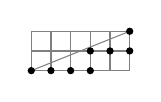
\begin{tikzpicture}
    \draw[step=0.25cm,color=gray] (0,0) grid (1.25,0.5);
    \draw[color=gray] (0,0) -- (1.25,0.5);
    \draw[fill=black] (0,0) circle (1.1pt);
    \draw[fill=black] (0.25,0) circle (1.1pt);
    \draw[fill=black] (0.5,0.0) circle (1.1pt);
    \draw[fill=black] (0.75,0.0) circle (1.1pt);
    \draw[fill=black] (0.75,0.25) circle (1.1pt);
    \draw[fill=black] (1,0.25) circle (1.1pt);
    \draw[fill=black] (1.25,0.25) circle (1.1pt);
    \draw[fill=black] (1.25,0.5) circle (1.1pt);
   \end{tikzpicture}.\\
   \raisebox{.55cm}{For $r_1=3$, $r_2=2$, $n=5$ we have $U_{n-3,1}=8$, $U_{n-4,2}=5$ so $R_n$ and $D_n$ are given by:} &
   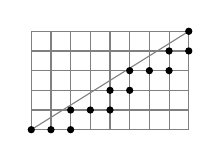
\begin{tikzpicture}
    \draw[step=0.25cm,color=gray] (0,0) grid (2,1.25);
    \draw[color=gray] (0,0) -- (2,1.25);
    \draw[fill=black] (0,0) circle (1.1pt);
    \draw[fill=black] (0.25,0) circle (1.1pt);
    \draw[fill=black] (0.5,0) circle (1.1pt);
    \draw[fill=black] (0.5,0.25) circle (1.1pt);
    \draw[fill=black] (0.75,0.25) circle (1.1pt);
    \draw[fill=black] (1,0.25) circle (1.1pt);
    \draw[fill=black] (1,0.5) circle (1.1pt);
    \draw[fill=black] (1.25,0.5) circle (1.1pt);
    \draw[fill=black] (1.25,0.75) circle (1.1pt);
    \draw[fill=black] (1.5,0.75) circle (1.1pt);
    \draw[fill=black] (1.75,0.75) circle (1.1pt);
    \draw[fill=black] (1.75,1) circle (1.1pt);
    \draw[fill=black] (2,1) circle (1.1pt);
    \draw[fill=black] (2,1.25) circle (1.1pt);
   \end{tikzpicture}.
  \end{tabular}\\

  \noindent We illustrate the compatible pairs in $\overline{\omega_H}$ as $\omega_H$ ranges over all horizontal gradings from \ref{def:compatibility} as well as give $x_{n-1}$ in these two cases.  When presenting $\overline{\omega_H}$ we indicate vertical edges in the support of $\omega_V$ with a black line labeled by $*s$ when $\omega_V$ may assign any value less than $s$.

  \begin{enumerate}
  \item For $r_1=5$, $r_2=1$, $n=5$ we have the following collections in $\cC(D_n)$ with corresponding monomials:\\
  \begin{tabular}{ccc}
   &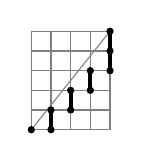
\begin{tikzpicture}
    \draw[step=0.25cm,color=gray] (0,0) grid (1,1.25);
    \draw[color=gray] (0,0) -- (1,1.25);
    \draw[color=black,line width=1.5pt] (0.25,0) -- (0.25,0.25);
    \draw[color=black,line width=1.5pt] (0.5,0.25) -- (0.5,0.5);
    \draw[color=black,line width=1.5pt] (0.75,0.5) -- (0.75,0.75);
    \draw[color=black,line width=1.5pt] (1,0.75) -- (1,1);
    \draw[color=black,line width=1.5pt] (1,1) -- (1,1.25);
    \draw[fill=black] (0,0) circle (1.1pt);
    \draw[fill=black] (0.25,0) circle (1.1pt);
    \draw[fill=black] (0.25,0.25) circle (1.1pt);
    \draw[fill=black] (0.5,0.25) circle (1.1pt);
    \draw[fill=black] (0.5,0.5) circle (1.1pt);
    \draw[fill=black] (0.75,0.5) circle (1.1pt);
    \draw[fill=black] (0.75,0.75) circle (1.1pt);
    \draw[fill=black] (1,0.75) circle (1.1pt);
    \draw[fill=black] (1,1) circle (1.1pt);
    \draw[fill=black] (1,1.25) circle (1.1pt);
   \end{tikzpicture} &
   \raisebox{.55cm}{\parbox{23cm}{$XYX^{-1}Y^{-1}\vdots X^{-1}P_2(X)XY^{-1}X^{-1}\vdots X^{-1}P_2(X)XY^{-1}X^{-1}\vdots  X^{-1}P_2(X)XY^{-1}X^{-1}\times\\\times X^{-1}P_2(X)XY^{-1}X^{-1}\vdots P_2(X)XY^{-1}X^{-1}$}}\\
  \end{tabular}
  Adding all of these terms gives $x_3=F_{P_1}F_{P_2}F_{P_1}(x)$.\\

  \item For $r_1=1$, $r_2=5$, $n=6$ we have the following collections in $\cC(D_n)$:\\
  \begin{tabular}{ccc}
   &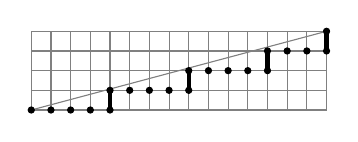
\begin{tikzpicture}
    \draw[step=0.25cm,color=gray] (0,0) grid (3.75,1);
    \draw[color=gray] (0,0) -- (3.75,1);
    \draw[color=black,line width=1.5pt] (1,0) -- (1,0.25);
    \draw[color=black,line width=1.5pt] (2,0.25) -- (2,0.5);
    \draw[color=black,line width=1.5pt] (3,0.5) -- (3,0.75);
    \draw[color=black,line width=1.5pt] (3.75,0.75) -- (3.75,1);
    \draw[fill=black] (0,0) circle (1.1pt);
    \draw[fill=black] (0.25,0) circle (1.1pt);
    \draw[fill=black] (0.5,0) circle (1.1pt);
    \draw[fill=black] (0.75,0) circle (1.1pt);
    \draw[fill=black] (1,0) circle (1.1pt);
    \draw[fill=black] (1,0.25) circle (1.1pt);
    \draw[fill=black] (1.25,0.25) circle (1.1pt);
    \draw[fill=black] (1.5,0.25) circle (1.1pt);
    \draw[fill=black] (1.75,0.25) circle (1.1pt);
    \draw[fill=black] (2,0.25) circle (1.1pt);
    \draw[fill=black] (2,0.5) circle (1.1pt);
    \draw[fill=black] (2.25,0.5) circle (1.1pt);
    \draw[fill=black] (2.5,0.5) circle (1.1pt);
    \draw[fill=black] (2.75,0.5) circle (1.1pt);
    \draw[fill=black] (3,0.5) circle (1.1pt);
    \draw[fill=black] (3,0.75) circle (1.1pt);
    \draw[fill=black] (3.25,0.75) circle (1.1pt);
    \draw[fill=black] (3.5,0.75) circle (1.1pt);
    \draw[fill=black] (3.75,0.75) circle (1.1pt);
    \draw[fill=black] (3.75,1) circle (1.1pt);
   \end{tikzpicture} &
   \raisebox{.45cm}{\parbox{23cm}{$XYX^{-1}Y^{-1}\vdots X^{-4}P_2(X)XY^{-1}X^{-1}\vdots X^{-4}P_2(X)XY^{-1}X^{-1}\times\\\times X^{-4}P_2(X)XY^{-1}X^{-1}\vdots X^{-3}P_2(X)XY^{-1}X^{-1}$}}\\
  \end{tabular}
  Adding all of these terms gives $x_5=F_1F_5F_1F_5F_1(x)$.\\
  \end{enumerate}

  \noindent Now a good exercise for the reader, which will help build intuition for the proof of Theorem~\ref{th:poly_positivity}, is to see how applying $F_1$ to the expression for $x_4$ with $r_1=5$, $r_2=1$ gives rise to the expression for $x_5$ with $r_1=1$, $r_2=5$.  Then compare with the proof of \cite[Lemma 9]{r1}.
 \end{example}
\begin{example}
 We present a pair of examples by which the reader can build their intuition for the proofs given in \cite{r1}.  These will be the cases $r_1=5$, $r_2=1$, $n=5$ and $r_1=1$, $r_2=5$, $n=6$.\\
 \begin{tabular}{cl}
  \raisebox{.55cm}{For $r_1=5$, $r_2=1$, $n=5$ we have $U_{n-3,1}=4$, $U_{n-4,2}=5$ so $R_n$ and $D_n$ are given by:} &
  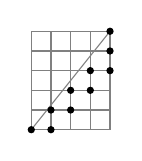
\begin{tikzpicture}
   \draw[step=0.25cm,color=gray] (0,0) grid (1,1.25);
   \draw[color=gray] (0,0) -- (1,1.25);
   \draw[fill=black] (0,0) circle (1.1pt);
   \draw[fill=black] (0.25,0) circle (1.1pt);
   \draw[fill=black] (0.25,0.25) circle (1.1pt);
   \draw[fill=black] (0.5,0.25) circle (1.1pt);
   \draw[fill=black] (0.5,0.5) circle (1.1pt);
   \draw[fill=black] (0.75,0.5) circle (1.1pt);
   \draw[fill=black] (0.75,0.75) circle (1.1pt);
   \draw[fill=black] (1,0.75) circle (1.1pt);
   \draw[fill=black] (1,1) circle (1.1pt);
   \draw[fill=black] (1,1.25) circle (1.1pt);
  \end{tikzpicture}.\\
  \raisebox{.45cm}{For $r_1=1$, $r_2=5$, $n=6$ we have $U_{n-3,1}=15$, $U_{n-4,2}=4$ so $R_n$ and $D_n$ are given by:} &
  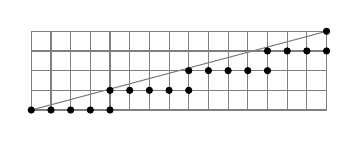
\begin{tikzpicture}
   \draw[step=0.25cm,color=gray] (0,0) grid (3.75,1);
   \draw[color=gray] (0,0) -- (3.75,1);
   \draw[fill=black] (0,0) circle (1.1pt);
   \draw[fill=black] (0.25,0) circle (1.1pt);
   \draw[fill=black] (0.5,0) circle (1.1pt);
   \draw[fill=black] (0.75,0) circle (1.1pt);
   \draw[fill=black] (1,0) circle (1.1pt);
   \draw[fill=black] (1,0.25) circle (1.1pt);
   \draw[fill=black] (1.25,0.25) circle (1.1pt);
   \draw[fill=black] (1.5,0.25) circle (1.1pt);
   \draw[fill=black] (1.75,0.25) circle (1.1pt);
   \draw[fill=black] (2,0.25) circle (1.1pt);
   \draw[fill=black] (2,0.5) circle (1.1pt);
   \draw[fill=black] (2.25,0.5) circle (1.1pt);
   \draw[fill=black] (2.5,0.5) circle (1.1pt);
   \draw[fill=black] (2.75,0.5) circle (1.1pt);
   \draw[fill=black] (3,0.5) circle (1.1pt);
   \draw[fill=black] (3,0.75) circle (1.1pt);
   \draw[fill=black] (3.25,0.75) circle (1.1pt);
   \draw[fill=black] (3.5,0.75) circle (1.1pt);
   \draw[fill=black] (3.75,0.75) circle (1.1pt);
   \draw[fill=black] (3.75,1) circle (1.1pt);
  \end{tikzpicture}.
 \end{tabular}\\

 \noindent We illustrate the compatible pairs in $\overline{\omega_H}$ as $\omega_H$ ranges over all horizontal gradings from \ref{def:compatibility} as well as give $x_{n-1}$ in these two cases.  When presenting $\overline{\omega_H}$ we indicate vertical edges in the support of $\omega_V$ with a black line labeled by $*s$ when $\omega_V$ may assign any value less than $s$.

 \begin{enumerate}
 \item For $r_1=5$, $r_2=1$, $n=5$ we have the following collections in $\cC(D_n)$ with corresponding monomials:\\
 \begin{tabular}{ccc}
  &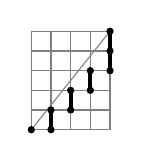
\begin{tikzpicture}
   \draw[step=0.25cm,color=gray] (0,0) grid (1,1.25);
   \draw[color=gray] (0,0) -- (1,1.25);
   \draw[color=black,line width=1.5pt] (0.25,0) -- (0.25,0.25);
   \draw[color=black,line width=1.5pt] (0.5,0.25) -- (0.5,0.5);
   \draw[color=black,line width=1.5pt] (0.75,0.5) -- (0.75,0.75);
   \draw[color=black,line width=1.5pt] (1,0.75) -- (1,1);
   \draw[color=black,line width=1.5pt] (1,1) -- (1,1.25);
   \draw[fill=black] (0,0) circle (1.1pt);
   \draw[fill=black] (0.25,0) circle (1.1pt);
   \draw[fill=black] (0.25,0.25) circle (1.1pt);
   \draw[fill=black] (0.5,0.25) circle (1.1pt);
   \draw[fill=black] (0.5,0.5) circle (1.1pt);
   \draw[fill=black] (0.75,0.5) circle (1.1pt);
   \draw[fill=black] (0.75,0.75) circle (1.1pt);
   \draw[fill=black] (1,0.75) circle (1.1pt);
   \draw[fill=black] (1,1) circle (1.1pt);
   \draw[fill=black] (1,1.25) circle (1.1pt);
  \end{tikzpicture} &
  \raisebox{.55cm}{\parbox{23cm}{$XYX^{-1}Y^{-1}\vdots X^{-1}P_2(X)XY^{-1}X^{-1}\vdots X^{-1}P_2(X)XY^{-1}X^{-1}\vdots X^{-1}P_2(X)XY^{-1}X^{-1}\times\\\times X^{-1}P_2(X)XY^{-1}X^{-1}\vdots P_2(X)XY^{-1}X^{-1}$}}\\
 \end{tabular}
 Adding all of these terms gives $x_4=F_5F_1F_5F_1(x)$.\\

 \item For $r_1=1$, $r_2=5$, $n=6$ we have the following collections in $\cC(D_n)$:\\
 \begin{tabular}{ccc}
  &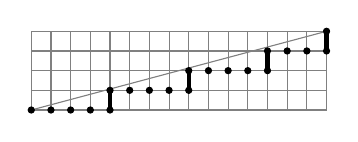
\begin{tikzpicture}
   \draw[step=0.25cm,color=gray] (0,0) grid (3.75,1);
   \draw[color=gray] (0,0) -- (3.75,1);
   \draw[color=black,line width=1.5pt] (1,0) -- (1,0.25);
   \draw[color=black,line width=1.5pt] (2,0.25) -- (2,0.5);
   \draw[color=black,line width=1.5pt] (3,0.5) -- (3,0.75);
   \draw[color=black,line width=1.5pt] (3.75,0.75) -- (3.75,1);
   \draw[fill=black] (0,0) circle (1.1pt);
   \draw[fill=black] (0.25,0) circle (1.1pt);
   \draw[fill=black] (0.5,0) circle (1.1pt);
   \draw[fill=black] (0.75,0) circle (1.1pt);
   \draw[fill=black] (1,0) circle (1.1pt);
   \draw[fill=black] (1,0.25) circle (1.1pt);
   \draw[fill=black] (1.25,0.25) circle (1.1pt);
   \draw[fill=black] (1.5,0.25) circle (1.1pt);
   \draw[fill=black] (1.75,0.25) circle (1.1pt);
   \draw[fill=black] (2,0.25) circle (1.1pt);
   \draw[fill=black] (2,0.5) circle (1.1pt);
   \draw[fill=black] (2.25,0.5) circle (1.1pt);
   \draw[fill=black] (2.5,0.5) circle (1.1pt);
   \draw[fill=black] (2.75,0.5) circle (1.1pt);
   \draw[fill=black] (3,0.5) circle (1.1pt);
   \draw[fill=black] (3,0.75) circle (1.1pt);
   \draw[fill=black] (3.25,0.75) circle (1.1pt);
   \draw[fill=black] (3.5,0.75) circle (1.1pt);
   \draw[fill=black] (3.75,0.75) circle (1.1pt);
   \draw[fill=black] (3.75,1) circle (1.1pt);
  \end{tikzpicture} &
  \raisebox{.45cm}{\parbox{23cm}{$XYX^{-1}Y^{-1}\vdots X^{-4}P_2(X)XY^{-1}X^{-1}\vdots X^{-4}P_2(X)XY^{-1}X^{-1}\times\\\times X^{-4}P_2(X)XY^{-1}X^{-1}\vdots X^{-3}P_2(X)XY^{-1}X^{-1}$}}\\
 \end{tabular}
 Adding all of these terms gives $x_5=F_1F_5F_1F_5F_1(x)$.\\
 \end{enumerate}

 \noindent Now a good exercise for the reader, which will help build intuition for the proofs in \cite{r1}, is to see how applying $F_1$ to the expression for $x_4$ with $r_1=5$, $r_2=1$ gives rise to the expression for $x_5$ with $r_1=1$, $r_2=5$.  Then compare with the proof of \cite[Lemma 9]{r1}.
\end{example}
 

%%%%%%%%%%%%%%%%%%%%%%%%%%%%%%%%%%%%%%%%%%%%%
\section{Combinatorics of Graded Compatible Pairs: Shadows}\label{sec:compatible pairs}

 Here we introduce our main combinatorial object of study, namely graded compatible pairs.  We will begin with general results that do not require an upper bound on the gradings and restrict to the bounded case when it becomes necessary.  Let $D=D_{a_1,a_2}$ be any maximal Dyck path with horizontal edges $H$ and vertical edges $V$.  

\subsection{Unbounded Gradings}
 \begin{definition}
  Consider functions $\omega_H:H\to\ZZ_{\ge0}$ and $\omega_V:V\to\ZZ_{\ge0}$ which we call \emph{horizontal} (resp. \emph{vertical}) \emph{gradings}.  We call the pair $(\omega_H,\omega_V)$ \emph{(graded) compatible} if for every $h\in H$ and $v\in V$ there exists an edge $e\in hv$ so that at least one of the following conditions on the gradings is satisfied:
  \begin{align}
   \label{eq:compatibility1}\tag{HGC} &\text{$e\ne v$}\quad\text{ and } \quad|(he)_V|=\sum\limits_{h'\in(he)_H}\omega_H(h');\\
   \label{eq:compatibility2}\tag{VGC} &\text{$e\ne h$}\quad\text{ and } \quad|(ev)_H|=\sum\limits_{v'\in(ev)_V}\omega_V(v').
  \end{align}
  Write $\cC=\cC_{a_1,a_2}$ for the set of all such compatible pairs $(\omega_H,\omega_V)$.
 \end{definition}
 \begin{remark}\label{rem:trivial_compatibility}
  For $h\in H$ with $\omega_H(h)=0$ the horizontal grading condition~\eqref{eq:compatibility1} of Definition~\ref{def:compatibility} is trivially satisfied for all $v\in V$ by taking $e=h$.  Similarly for $v\in V$ with $\omega_V(v)=0$ the vertical grading condition~\eqref{eq:compatibility2} is trivially satisfied.
 \end{remark}

 In order to prove Theorem~\ref{th:poly_positivity} we will need to develop some of the combinatorics of compatible pairs, many of the results from this section are generalizations of, or are inspired by, similar results from \cite[Section 3]{llz}.  

 For a horizontal grading $\omega_H:H\to\ZZ_{\ge0}$, write $\overline{\omega_H}$ for the set of all vertical gradings $\omega_V:V\to\ZZ_{\ge0}$ with $(\omega_H,\omega_V)\in\cC$.  Define $\overline{\omega_V}$ similarly.  We define the \emph{magnitude} of a horizontal grading $\omega_H$ or a vertical grading $\omega_V$ respectively by $|\omega_H|=\sum\limits_{h\in H}\omega_H(h)$ and $|\omega_V|=\sum\limits_{v\in V} \omega_V(v)$.  The following result greatly simplifies the check for membership in $\overline{\omega_H}$ and $\overline{\omega_V}$.
 \begin{lemma}\label{le:shadows}\mbox{}
  \begin{enumeratea}
   \item For every $\omega_H:H\to\ZZ_{\ge0}$ there exist subsets $\rsh(\omega_H)\subset\sh(\omega_H)\subset V$ such that:
   \begin{enumeratei}
    \item for $\omega_V:V\to\ZZ_{\ge0}$, $\omega_V\in\overline{\omega_H}$ if and only if $\omega_V(v)=0$ for all $v\in\sh(\omega_H)\setminus\rsh(\omega_H)$ and one of the conditions \eqref{eq:compatibility1} or \eqref{eq:compatibility2} is satisfied for each $h\in\supp(\omega_H)$ and $v\in\rsh(\omega_H)$;
    \item $|\sh(\omega_H)|=\min(a_2,|\omega_H|)$.
   \end{enumeratei}
   \item For every $\omega_V:V\to\ZZ_{\ge0}$ there exist subsets $\rsh(\omega_V)\subset\sh(\omega_V)\subset H$ such that
   \begin{enumeratei}
    \item for $\omega_H:H\to\ZZ_{\ge0}$, $\omega_H\in\overline{\omega_V}$ if and only if $\omega_H(h)=0$ for all $h\in\sh(\omega_V)\setminus\rsh(\omega_V)$ and one of the conditions \eqref{eq:compatibility1} or \eqref{eq:compatibility2} is satisfied for each $h\in\rsh(\omega_V)$ and $v\in\supp(\omega_V)$;
    \item $|\sh(\omega_V)|=\min(a_1,|\omega_V|)$.
   \end{enumeratei}
  \end{enumeratea}
 \end{lemma}

 We will refer to the sets $\sh(\omega_H)$ and $\rsh(\omega_H)$ respectively as the \emph{shadow} and \emph{remote shadow} of $\omega_H$ (and similarly for $\omega_V$).  Before proving Lemma~\ref{le:shadows} we require some preparation.  The shadow of each $\omega_H$ will be defined in terms of certain ``local shadows''.
 \begin{definition}\label{def:local}\mbox{}
  \begin{enumeratea}
   \item For each $h\in H$, define $\sh(h;\omega_H)$, the \emph{local shadow of $\omega_H$ at $h$}, as the set of vertical edges $(he)_V$ in the shortest subpath $he$ of $D$ such that $|(he)_V|=\sum\limits_{h'\in(he)_H}\omega_H(h')$.  Write $D(h;\omega_H)=he$ for this minimal path.  If there is no such subpath then we set $\sh(h;\omega_H)=V$ and $D(h;\omega_H)=D$.  We define the \emph{shadow} of $\omega_H$ as the union of local shadows: $\sh(\omega_H)=\bigcup\limits_{h\in H}\sh(h;\omega_H)$.
   \item For each $v\in V$, define $\sh(v;\omega_V)$, the \emph{local shadow of $\omega_V$ at $v$}, as the set of horizontal edges $(ev)_H$ in the shortest subpath $ev$ of $D$ such that $|(ev)_H|=\sum\limits_{v'\in(ev)_V}\omega_V(v')$.  Write $D(v;\omega_V)$ for this minimal path $ev$.  If there is no such subpath then we set $\sh(v;\omega_V)=H$ and $D(v;\omega_V)=D$.  We define the \emph{shadow} of $\omega_V$ as the union of local shadows: $\sh(\omega_V)=\bigcup\limits_{v\in V}\sh(v;\omega_V)$.
  \end{enumeratea}
 \end{definition}
 \begin{remark}
  When $\omega_H(h)=0$, we have $\sh(h;\omega_H)=\emptyset$ and $D(h;\omega_H)=hh$ is the subpath of $D$ consisting of only the edge $h$.  A similar claim holds if $\omega_V(v)=0$.
 \end{remark}

 It will be useful to consider certain \emph{shadow statistics} for subpaths of $D$ which are closely related to the compatibility conditions for a pair $(\omega_H,\omega_V)\in\cC$.  
 \begin{definition}\label{def:shadow statistics}
  For a subpath $ee'\subset D$ define the \emph{horizontal shadow statistic}
  \[f_{\omega_H}(ee'):=-|(ee')_V|+\sum\limits_{h\in(ee')_H}\omega_H(h)\]
  for each horizontal grading $\omega_H$ and the \emph{vertical shadow statistic}
  \[f_{\omega_V}(ee'):=-|(ee')_H|+\sum\limits_{v\in(ee')_V}\omega_V(v)\]
  for each vertical grading $\omega_V$.  
 \end{definition}
 It immediately follows from the definitions that the functions $f_{\omega_H}$ and $f_{\omega_V}$ satisfy the following additivity property with respect to concatenation of paths:
 \begin{align*}
  f_{\omega_H}(ee''')&=f_{\omega_H}(ee')+f_{\omega_H}(e''e'''),\\
  f_{\omega_V}(ee''')&=f_{\omega_V}(ee')+f_{\omega_V}(e''e'''),
 \end{align*}
 whenever $ee'''=ee'\amalg e''e'''$.  For each subpath $ee'\subset D$ we obtain a factor $X_{\omega_H,\omega_V}(ee')$ of the monomial $X_{\omega_H,\omega_V}$ by multiplying the weights of edges along the path $ee'$.
 \begin{lemma}
  The quantities $f_{\omega_H}(ee')$ and $f_{\omega_V}(ee')$ record the total $Y$-degree and the total $X$-degree respectively of the monomial $X_{\omega_H,\omega_V}(ee')$.
 \end{lemma}
 \begin{proof}
  A horizontal edge $h\in(ee')_H$ contributes a factor of $p_{\omega_H(h)}Y^{\omega_H(h)}X^{-1}$ to $X_{\omega_H,\omega_V}(ee')$ while a vertical edge $v\in(ee')_V$ contributes a factor of $p'_{\omega_V(v)}X^{\omega_V(v)+1}Y^{-1}X^{-1}$.  The result now follows by comparing the total $Y$- and $X$-degrees of $X_{\omega_H,\omega_V}(ee')$ with the definitions of $f_{\omega_H}(ee')$ and $f_{\omega_V}(ee')$ respectively.
 \end{proof}
 The next lemma relates the minimal shadow paths $D(h;\omega_H)$ and $D(v;\omega_V)$ to the shadow statistics.
 \begin{lemma}\label{le:sub_compatibility}\mbox{}
  \begin{enumeratea}
   \item Suppose $h\in\supp(\omega_H)$ and write $D(h;\omega_H)=he$.
   \begin{enumeratei}
    \item $f_{\omega_H}(D(h;\omega_H))=0$.
    \item For any proper subpath $he'\subset D(h;\omega_H)$ we have $f_{\omega_H}(he')>0$.
    \item For any proper subpath $e'e\subset D(h;\omega_H)$ we have $f_{\omega_H}(e'e)<0$.
   \end{enumeratei}
   In particular, one may conclude that the last edge $e$ of $D(h;\omega_H)$ is vertical.
   \item Suppose $v\in\supp(\omega_V)$ and write $D(v;\omega_V)=ev$.
   \begin{enumeratei}
    \item $f_{\omega_V}(D(v;\omega_V))=0$.
    \item For any proper subpath $e'v\subset D(v;\omega_V)$ we have $f_{\omega_V}(e'v)>0$.
    \item For any proper subpath $ee'\subset D(v;\omega_V)$ we have $f_{\omega_V}(ee')<0$.
   \end{enumeratei}
   In particular, one may conclude that the first edge $e$ of $D(v;\omega_V)$ is horizontal.
  \end{enumeratea}
 \end{lemma}
 
 The next easy result is an immediate consequence of Lemma~\ref{le:sub_compatibility} but exhibits a strong influence on the results below.
 \begin{corollary}\label{cor:remote_shadow_compatibility}
  Suppose $h\in\supp(\omega_H)$ and let $v\in D(h;\omega_H)$ be any vertical edge.  Then (HC) is not satisfied for $h$ and $v$, however for any $\omega_V\in\overline{\omega_H}$ the condition (VC) is satisfied for $h$ and $v$.  In particular, $D(v;\omega_V)$ is a proper subpath of $hv$.
 \end{corollary}

 We can now understand the relationships between the various local shadows associated to a horizontal grading $\omega_H$ or a vertical grading $\omega_V$.
 \begin{lemma}\label{le:shadow containment}\mbox{}
  \begin{enumeratea}
   \item Let $\omega_H$ be a horizontal grading.  For any horizontal edges $h,h'\in H$, the local shadows $\sh(h;\omega_H)$ and $\sh(h';\omega_H)$ are either disjoint or one is contained in the other.
   \item Let $\omega_V$ be a vertical grading.  For any vertical edges $v,v'\in V$, the local shadows $\sh(v;\omega_V)$ and $\sh(v';\omega_V)$ are either disjoint or one is contained in the other.
  \end{enumeratea}
 \end{lemma}
 
 It follows from Lemma~\ref{le:shadow containment} that for any fixed horizontal grading $\omega_H$ we can find horizontal edges $\eta_1,\ldots,\eta_p\in H$ (labeled in the natural order along the Dyck path $D$) such that
 \begin{itemize}
  \item $\omega_H(\eta_j)>0$ for $1\le j\le p$;
  \item $\sh(\eta_i;\omega_H)\cap\sh(\eta_j;\omega_H)=\emptyset$ for $i\ne j$;
  \item $\sh(\omega_H)=\sh(\eta_1;\omega_H)\amalg\cdots\amalg\sh(\eta_p;\omega_H)$ is a partition of $\sh(\omega_H)$.
 \end{itemize}
 Define vertical edges $\nu_1,\ldots,\nu_p$ by $D(\eta_j;\omega_H)=\eta_j\nu_j$.
   
 Our ultimate proof of Theorem~\ref{th:poly_positivity} will be achieved by restricting attention to these maximal local shadows.

 \begin{definition}\mbox{}
  \begin{enumeratea}
   \item The \emph{remote shadow} of $\omega_H$ is the set $\rsh(\omega_H)$ obtained from $\sh(\omega_H)$ by removing for each $d\in[1,a_1]$ the (up to) $\omega_H(h_d)$ vertical edges of depth $d$ immediately following $h_d$.  By considering the definition of compatibility one may alternatively described $\rsh(\omega_H)\subset\sh(\omega_H)$ as the subset consisting of all vertical edges $v$ for which there exists a vertical grading $\omega_V\in\overline{\omega_H}$ with $\omega_V(v)\ne0$.
   \item The \emph{remote shadow} of $\omega_V$ is the set $\rsh(\omega_V)$ obtained from $\sh(\omega_V)$ by removing for each $\ell\in[1,a_2]$ the (up to) $\omega_V(v_\ell)$ horizontal edges of height $\ell-1$ immediately preceding $v_\ell$.  By considering the definition of compatibility one may alternatively describe $\rsh(\omega_V)\subset\sh(\omega_V)$ as the subset consisting of all horizontal edges $h$ for which there exists a horizontal grading $\omega_H\in\overline{\omega_V}$ with $\omega_H(h)\ne0$.
  \end{enumeratea}
 \end{definition}
 
 It will be useful to partition the remote shadows according to which local shadow contains a given edge. 
 \begin{definition}\label{def:remote_shadows}\mbox{}
  \begin{enumeratea}
   \item For $0<j\le a_1$ and $0<d\le a_1$, denote by $\rsh(\omega_H)_{j;d}$ the set of $v\in\rsh(\omega_H)$ of depth $d$ such that $v\in\sh(h_j;\omega_H)$ and $h_j$ is the first edge before $v$ with this property (i.e. the path $h_jv$ is shortest possible).  Define the \emph{local remote shadow} of the edge $h_j$ as $\rsh(h_j;\omega_H)=\coprod\limits_{d\in[1,a_1]}\rsh(\omega_H)_{j;d}$.
   \item For $0<k\le a_2$ and $0\le \ell<a_2$, denote by $\rsh(\omega_V)_{k;\ell}$ the set of $h\in\rsh(\omega_V)$ of height $\ell$ such that $h\in\sh(v_k;\omega_V)$ and $v_k$ is the first edge after $h$ with this property (i.e. the path $hv_k$ is shortest possible).  Define the \emph{local remote shadow} of the edge $v_k$ as $\rsh(v_k;\omega_V)=\coprod\limits_{\ell\in[0,a_2-1]}\rsh(\omega_V)_{k;\ell}$.
  \end{enumeratea}
 \end{definition}
 \begin{remark}\label{rem:remote_shadow_decomposition}
  For a horizontal grading $\omega_H$ there are only finitely many $j$ with $\rsh(h_j;\omega_H)\ne\emptyset$.  Thus there exists a sequence $1\le j_1<\cdots<j_n\le a_1$ such that $\rsh(h_{j_t};\omega_H)\ne\emptyset$ for each $t\in[1,n]$ and there is a partition $\rsh(\omega_H)=\rsh(h_{j_1};\omega_H)\amalg\cdots\amalg\rsh(h_{j_n};\omega_H)$.
 \end{remark}

 The next lemma gives precise conditions describing when the remote shadows $\rsh(\omega_H)_{j;d}$ and $\rsh(\omega_V)_{j;\ell}$ are non-empty.  First note that $\rsh(\omega_H)_{d;d}=\emptyset$ for every $d$ and $\rsh(\omega_V)_{\ell+1;\ell}=\emptyset$ for every $\ell$.
 \begin{lemma}\label{le:remote_shadow_conditions}\mbox{}
  \begin{enumeratea}
   \item Let $0<d,j\le a_1$ with $j\ne d$.  Then $\rsh(\omega_H)_{j;d}\ne\emptyset$ if and only if $f_{\omega_H}(h_j\overline{h})>0>f_{\omega_H}(h\overline{h}_{d+1})$ for every horizontal edge $h\in (\overline{h}_j\overline{h}_{d+1})_H$.
   \item Let $0\le\ell< a_2$ and $0<j\le a_2$ with $j\ne\ell+1$.  Then $\rsh(\omega_V)_{j;\ell}\ne\emptyset$ if and only if $f_{\omega_V}(\overline{v}_\ell v)<0<f_{\omega_V}(\overline{v}v_j)$ for every vertical edge $v\in (\overline{v}_\ell\overline{v}_j)_V$.
  \end{enumeratea}
 \end{lemma}
 \begin{remark}
  The inequalities above imply that when $\rsh(\omega_H)_{j;d}\ne\emptyset$ the set $\rsh(\omega_H)_{j';d'}$ will be empty whenever $j<j'<d<d'$.
 \end{remark}


 Now we are able to give an explicit formula for the sizes of the remote shadows.
 \begin{lemma}\label{le:remote_shadow_sizes}\mbox{}
  \begin{enumeratea}
   \item Let $0<d,j\le a_1$ with $d\ne j$ and suppose $f_{\omega_H}(h_j\overline{h})>0>f_{\omega_H}(h\overline{h}_{d+1})$ for every horizontal edge $h\in (\overline{h}_j\overline{h}_{d+1})_1$.  Then $|\rsh(\omega_H)_{j;d}|=\min\limits_{h\in (\overline{h}_j\overline{h}_{d+1})_1}\min\big(f_{\omega_H}(h_j\overline{h}),-f_{\omega_H}(h\overline{h}_{d+1})\big)$.
   \item Let $0\le\ell< a_2$ and $0<j\le a_2$ with $\ell\ne j$ and suppose $f_{\omega_V}(\overline{v}_\ell v)<0<f_{\omega_V}(\overline{v}v_j)$ for every vertical edge $v\in (\overline{v}_\ell\overline{v}_j)_2$.  Then $|\rsh(\omega_V)_{j;\ell}|=\min\limits_{v\in (\overline{v}_\ell\overline{v}_j)_2}\min\big(-f_{\omega_V}(\overline{v}_\ell v),f_{\omega_V}(\overline{v}v_j)\big)$.
  \end{enumeratea}
 \end{lemma}

 The constructions and results below do not come from \cite{llz}.  We will need to introduce partial orders on the sets $\overline{\omega_H}$ and $\overline{\omega_V}$.
 \begin{definition}\label{def:partial_order}\mbox{}
  \begin{enumeratea}
   \item For each horizontal grading $\omega_H:H\to\ZZ_{\ge0}$, define a partial order on $\overline{\omega_H}$ by $\omega_V\le \omega'_V$ if $\omega_V(v)\le\omega'_V(v)$ for all $v\in V$, equivalently $\omega_V\le\omega'_V$ if $f_{\omega_V}(ee')\le f_{\omega'_V}(ee')$ for every subpath $ee'\subset D$.
   \item For each vertical grading $\omega_V:V\to\ZZ_{\ge0}$, define a partial order on $\overline{\omega_V}$ by $\omega_H\le \omega'_H$ if $\omega_H(h)\le\omega'_H(h)$ for all $h\in H$, equivalently $\omega_H\le\omega'_H$ if $f_{\omega_H}(ee')\le f_{\omega'_H}(ee')$ for every subpath $ee'\subset D$.
  \end{enumeratea}
 \end{definition}

 Following Lemma~\ref{le:shadows} the compatibility of a pair $(\omega_H,\omega_V)$ is completely controlled by $\supp(\omega_V)\cap\rsh(\omega_H)$.  Write $\overline{\omega_H}^{rs}\subset\overline{\omega_H}$ for the subset containing all $\omega_V$ with $\supp(\omega_V)\subset\rsh(\omega_H)$.  Define $\overline{\omega_V}^{rs}$ similarly.

 \begin{lemma}\label{lem:shadow_magnitude}
  For any $\omega_V\in\overline{\omega_H}^{rs}$ we have $\sh(\omega_V)\ne H$ and $|\sh(\omega_V)|=|\omega_V|$.
 \end{lemma}

 Write $\Max(\overline{\omega_H})$ for the set of maximal elements of $\overline{\omega_H}$ under the partial order $\le$.  Define $\Max(\overline{\omega_V})$ similarly.
 \begin{definition}
  Define a ``revlex'' total order on $\Max(\overline{\omega_H})$ by $\omega_V\prec\omega'_V$ if there exists $j\in[0,a_2-1]$ such that $\omega_V(v_{a_2-i+1})=\omega'_V(v_{a_2-i+1})$ for $i\in[1,j]$ but $\omega_V(v_{a_2-j})<\omega'_V(v_{a_2-j})$, equivalently $\omega_V\prec\omega'_V$ if there exists $j\in[1,a_2]$ such that $f_{\omega_V}(ev_{a_2})=f_{\omega'_V}(ev_{a_2})$ for every $e\in\overline{v}_jv_{a_2}$ but $f_{\omega_V}(v_jv_{a_2})<f_{\omega'_V}(v_jv_{a_2})$.  Write $\omega_V^{(1)}\succ \omega_V^{(2)}\succ\cdots\succ \omega_V^{(n)}$ for the elements of $\Max(\overline{\omega_H})$.
 \end{definition}
 \begin{remark}
  The minimal element of $\Max(\overline{\omega_H})$ under $\prec$ is obtained by reading the vertical edges in the natural order along $D$ and sequentially assigning each edge the maximal possible grade which maintains compatibility.  The maximal element of $\Max(\overline{\omega_H})$ is obtained by the same procedure but reading the vertical edges in reverse order.
 \end{remark}

 Consider the decomposition $\rsh(\omega_H)=\rsh(h_{j_1};\omega_H)\amalg\cdots\amalg\rsh(h_{j_n};\omega_H)$ from Remark~\ref{rem:remote_shadow_decomposition}.  Write $d_p$ for the ``deepest'' depth appearing in the shadow of $h_{j_p}$, i.e. the index $d_p$ such that 
 \[(h_{j_p}h_{d_p})_1=\max\limits_{d:\rsh(\omega_H)_{j_p;d}\ne\emptyset}(h_{j_p}h_d)_1.\]
 Let $\omega_V\in\Max(\overline{\omega_H}^{rs})$.  Each component $\rsh(h_{j_p};\omega_H)$ must contain a vertical edge $v\in\supp(\omega_V)$ for otherwise we could construct from $\omega_V$ a vertical grading with larger magnitude, contradicting maximality.  Since $\sh(\omega_V)\ne H$ it follows from Lemma~\ref{le:shadow containment} that there exist sequences $(\beta_{1,1},\ldots,\beta_{1,m_1}),\ldots,(\beta_{n,1},\ldots,\beta_{n,m_n})$ satisfying the following conditions:
 \begin{itemize}
  \item $v_{\beta_{p,\ell}}\in\supp(\omega_V)\cap\rsh(h_{j_p};\omega_H)$;
  \item $(h_{j_p}v_{\beta_{p,\ell}})_2<(h_{j_p}v_{\beta_{p,\ell'}})_2$ for $\ell<\ell'$;
  \item $\sh(\omega_V)=\sh(v_{\beta_{1,1}};\omega_V)\amalg\cdots\amalg\sh(v_{\beta_{1,m_1}};\omega_V)\amalg\cdots\amalg\sh(v_{\beta_{n,1}};\omega_V)\amalg\cdots\amalg\sh(v_{\beta_{n,m_n}};\omega_V)$.
 \end{itemize}
 \begin{lemma}
  For each $p$ we have $v_{\beta_{p,m_p}}\in\rsh(\omega_H)_{j_p;d_p}$ and thus the value $(h_{j_p+1}v_{\beta_{p,m_p}})_1=(h_{j_p+1}h_{d_p})_1$ is independent of the choice of $\omega_V\in\Max(\overline{\omega_H}^{rs})$.
 \end{lemma}
 \begin{proof}
  By the definition of $d_p$ we have $v_{\beta_{p,m_p}}\in\rsh(\omega_H)_{j_p;d}$ for some $d$ with $(h_{j_p}h_d)_1\le(h_{j_p}h_{d_p})_1$.  If the inequality was strict, any edge $v\in\rsh(\omega_H)_{j_p;d_p}$ would satisfy $\omega_V(v)=0$.  Then taking an edge $v\in\rsh(\omega_H)_{j_p;d_p}$ and increasing the value of $\omega_V$ on $v$ to 1 does not affect compatibility, but this contradicts the maximality of $\omega_V$.
 \end{proof}
  
 \begin{corollary}\label{cor:maximal_shadows}\mbox{}
  \begin{enumeratea}
   \item For any $\omega_V,\omega'_V\in\Max(\overline{\omega_H}^{rs})$ we have 
   \[|\omega_V|=|\omega'_V|=\sum\limits_{p=1}^n(h_{j_p+1}h_{d_p})_1.\]
   \item If $\omega_H,\omega'_H\in\Max(\omega_V)$ are maximal elements of $\cC_{rs}(\omega_V)$ then 
   \[|\omega_H|=|\omega'_H|=(\overline{v}_{\ell'_1}v_{\beta'_1})_2+\cdots+(\overline{v}_{\ell'_n}v_{\beta'_n})_2.\]
  \end{enumeratea}
 \end{corollary}
 \begin{proof}
  For $1\le p\le n$, the minimal shadow path $D(v_{\beta_{p,\ell}};\omega_V)$ is a proper subpath of $h_{j_p}v_{\beta_{p,\ell}}$ for each $\ell$.  Moreover, the decomposition of $\sh(\omega_V)$ above implies the paths $D(v_{\beta_{p,\ell}};\omega_V)$ and $D(v_{\beta_{p,\ell'}};\omega_V)$ are disjoint for $\ell\ne\ell'$.  By maximality of $\omega_V$ we have a decomposition $h_{j_p+1}v_{\beta_{p,m_p}}=D(v_{\beta_{p,1}};\omega_V)\amalg\cdots\amalg D(v_{\beta_{p,m_p}};\omega_V)$ which implies 
  $(h_{j_p+1}v_{\beta_{p,m_p}})_1=\sum\limits_{\ell=1}^{m_p}|\sh(v_{\beta_{p,\ell}};\omega_V)|$.  It then follows from Lemma~\ref{lem:shadow_magnitude} that
  \[|\omega_V|=|\sh(\omega_V)|=\sum\limits_{p=1}^n\sum\limits_{\ell=1}^{m_p}|\sh(v_{\beta_{p,\ell}};\omega_V)|=\sum\limits_{p=1}^n(h_{j_p+1}v_{\beta_{p,m_p}})_1=\sum\limits_{p=1}^n(h_{j_p+1}h_{d_p})_1.\]
 \end{proof}

 \begin{proposition}
  Characterization of $\Max(\overline{\omega_H}^{rs})$ as sequences of non-negative integers satisfying some conditions...
 \end{proposition}

 Suppose $\sh(h_{j_\ell};\omega_H)\supset\sh(h_{j_p};\omega_H)$ with $\ell<p$.  Then for any $v_{\beta_{\ell,i}}$ which comes after $\sh(h_{j_p};\omega_H)$ we must have $\omega_V(v_{\beta_{\ell,i}})$ is maximal.

 \subsection{Left-Justified Horizontal Gradings}
 We will call a horizontal grading $\omega_H:H\to\ZZ_{\ge0}$ \emph{left-justified} if there exists $j\in[0,a_1]$ such that $\omega_H(h_\ell)>0$ for $\ell\in[1,j]$ and $\omega_H(h_\ell)=0$ otherwise.
 \begin{lemma}
  Suppose $\omega_H$ is left-justified.  Then $|\rsh(\omega_H)|=|\sh(\omega_H)|-\left\lfloor\frac{|\supp(\omega_H)|a_2}{a_1}\right\rfloor$.
 \end{lemma}
 \begin{proof}
  The quantity $\left\lfloor\frac{|\supp(\omega_H)|a_2}{a_1}\right\rfloor$ is exactly the number of vertical edges in $\sh(\omega_H)\setminus\rsh(\omega_H)$, the result follows.
 \end{proof}
 
 Let $\omega_H$ be left-justified and abbreviate $h(\omega_H)=\left\lfloor\frac{|\supp(\omega_H)|a_2}{a_1}\right\rfloor$ and $s_j=|\{i\st v_{h(\omega_H)+j}\in\sh(h_i;\omega_H)\}|$.  Write $W(\omega_H)\subset\ZZ_{\ge0}^{|\rsh(\omega_H)|}$ for the subset of all sequences $\big(w_1,\ldots,w_{|\rsh(\omega_H)|}\big)$ satisfying the following two conditions:
 \begin{enumeratei}
  \item $\sum\limits_{i=1}^j w_i\le\left\lceil\frac{(h(\omega_H)+j)a_1}{a_2}\right\rceil-s_j$ for $j\in\big[1,|\rsh(\omega_H)|-1\big]$;
  \item $\sum\limits_{i=1}^{|\rsh(\omega_H)|} w_i=\left\lceil\frac{|\sh(\omega_H)|a_1}{a_2}\right\rceil-s_{|\rsh(\omega_H)|}$.
 \end{enumeratei}
 \begin{proposition}
  For left-justified $\omega_H$ there is a bijection $\Max(\overline{\omega_H}^{rs})\to W(\omega_H)$.
 \end{proposition}
 \begin{proof}
  According to Lemma~\ref{le:height_depth} the quantity $\left\lceil\frac{(h(\omega_H)+j)a_1}{a_2}\right\rceil$ is exactly the depth of the vertical edge $v_{h(\omega_H)+j}$.  In order to have compatibility we need the local shadow of $v_{h(\omega_H)+j}$ to be properly contained in the local shadow path $D(h_i;\omega_H)$ whenever $v_{h(\omega_H)+j}\in\sh(h_i;\omega_H)$ by Corollary~\ref{cor:remote_shadow_compatibility}.  In particular, whenever $v_{h(\omega_H)+j}\in\sh(h_i;\omega_H)$ we must have $h_i\notin\sh(v_{h(\omega_H)+j};\omega_V)$ which gives the inequality $\sum\limits_{i=1}^j w_i\le\left\lceil\frac{(h(\omega_H)+j)a_1}{a_2}\right\rceil-s_j$ for each $j\in[1,|\rsh(\omega_H)|$.  By maximality of $\omega_V$ this inequality must be an equality for $j=|\rsh(\omega_H)|$.
 \end{proof}

 A maximal vertical grading $V\in\Max(\overline{\omega_H}^{rs})$ will be called \emph{left-justified} if it corresponds to the unique element of $W(\omega_H)$ for which every inequality in (i) is an equality.\\

 We will call an $r_1$-bounded vertical grading $\omega_H$ \emph{fully left-justified} if $\omega_H$ is left-justified and $\omega_H(h_i)=r_1$ for every $h_i\in\supp(\omega_H)$.
 



 \ \\
 \ \\
 \ \\

 Write $s=|\supp(\omega_H)|$.  Define the sequence $1\le d_1<\cdots<d_s\le a_1$ and an element $\epsilon\in\{0,1\}^s$ such that $\supp(\omega_H)=\{h_{d_1},\ldots,h_{d_s}\}$ and $\epsilon_i=1$ whenever $\rsh(h_{d_i};\omega_H)\ne\emptyset$.  

 \newpage

 We will extend the notation $\beta_{i,\ell}$ to label all of the vertical edges of depth $i$.  Write 
 \[\sigma(i)=\min\big(\omega_H(h_i),\lfloor ia_2/a_1\rfloor-\lfloor (i-1)a_2/a_1\rfloor\big).\]
 Then for $\ell\in[-\sigma(i)+1,0]$ we will denote by $v_{\beta_{i,\ell}}$ the vertical edges of depth $i$ from $\sh(\omega_H)\setminus\rsh(\omega_H)$ where the labeling matches the natural order along $D$.  For $\ell\in[m_i+1,\lfloor ia_2/a_1\rfloor-\lfloor (i-1)a_2/a_1\rfloor$ we will write $v_{\beta_{i,\ell}}$ for an edge of depth $i$ which lies beyond the shadow of $\omega_H$, again labeling in the natural order along $D$.

 
 \fbox{For any $\omega_V\in\overline{\omega_H}$ we have $X_{\omega_H,\omega_V}(h_jv_{\beta_{j,0}})=p_{\omega_H(h_j)}Y^{\omega_H(h_j)-\sigma(j)}X^{-1}$.}\\

 \fbox{If there exists $d$ with $\rsh(\omega_H)_{j;d}\ne\emptyset$ then $\omega_H(h_j)-\sigma(j)>0$.}\\

 Following Definition~\ref{def:remote_shadows} the remote shadow also breaks up into a disjoint union of connected intervals \[\rsh(\omega_H)=\coprod\limits_{j\in\supp(\omega_H),d\in[1,a_1]}\rsh(\omega_H)_{j;d}.\]
 It will be useful to consider all edges of fixed depth $d\in[1,a_1]$ in the remote shadow 
 \[\rsh(\omega_H)_d:=\coprod\limits_{j\in\supp(\omega_H)}\rsh(\omega_H)_{j;d}.\]  
 Then the depth $d$ shadow of $\omega_H$ is the connected interval 
 \[\sh(\omega_H)_d:=I_d\amalg\rsh(\omega_H)_d=\{v_{d;1},\ldots,v_{d;\ell(d)}\}\]
 so that $\sh(\omega_H)=\coprod\limits_{d=1}^{a_1}\sh(\omega_H)_d$.

 Write $s=|\supp(\omega_H)|$ and $t=|\rsh(\omega_H)|=\sum\limits_{d=1}^{a_1}(\ell(d)-\sigma(d))$.  Consider the sequences $1\le d_1<\cdots<d_s\le a_1$ and $1\le j_1<\cdots<j_t\le a_2$ such that $\supp(\omega_H)=\{h_{d_1},\ldots,h_{d_s}\}$ and $\rsh(\omega_H)=\{v_{j_1},\ldots,v_{j_t}\}$.  Define the ``gap sequences'' $1\le\alpha_i,\delta_i\le t$ for $i\in[1,s]$ satisfying the following three properties:
 \begin{itemize}
  \item $\alpha_1\le\delta_1<\alpha_2\le\delta_2<\cdots<\alpha_{s-1}\le\delta_{s-1}$;
  \item $\coprod\limits_{d=d_p}^{d_{p+1}-1}\rsh(\omega_H)_d=\{v_{j_{\alpha_p}},\ldots,v_{j_{\delta_p}}\}$ for $p\in[1,s-1]$;
  \item $\coprod\limits_{d=d_s}^{a_1}\rsh(\omega_H)_d\amalg\coprod\limits_{d=1}^{d_1-1}\rsh(\omega_H)_d=\{v_{j_{\alpha_s}},\ldots,v_{j_t}\}\amalg\{v_{j_1},\ldots,v_{j_{\delta_s}}\}$.
 \end{itemize}
 It follows that $v_{j_{\alpha_p}}v_{j_{\delta_p}}$ is a proper subpath of $h_{d_p}\overline{h}_{d_{p+1}}$ for $p\in[1,s-1]$ and $v_{j_{\alpha_s}}v_{j_{\delta_s}}$ is a proper subpath of $h_{d_s}\overline{h}_{d_1}$.  In particular $\supp(\omega_H)\cap(v_{j_{\alpha_p}}v_{j_{\delta_p}})_1=\emptyset$ for every $p\in[1,s]$ and $\supp(\omega_H)\cap(v_{j_{\delta_p}}v_{j_{\alpha_{p+1}}})_1\ne\emptyset$ for $p\in[1,s-1]$.

 Looking again at the definition of $M_i(\omega_H)$ we see that there exists an ``equality cut-off'' sequence $\gamma_1,\ldots,\gamma_s$ such that 
 \begin{itemize}
  \item $\alpha_p\le\gamma_p\le\delta_p$ for $p\in[1,s]$;
  \item for each $\omega_V\in M_i(\omega_H)$ we have $\omega_V(v_{j_\beta})=\omega_V^{(i)}(v_{j_\beta})$ for each $\beta\in E$ where $E:=[\alpha_1,\gamma_1-1]\cup\cdots\cup[\alpha_t,\gamma_t-1]$ is the ``equality set'' of $M_i(\omega_H)$;
  \item for $\beta\in[1,s]\setminus E$ and $d\le \omega_V^{(i)}(v_{j_\beta})$ there exists $\omega_V\in M_i(\omega_H)$ with $\omega_V(v_{j_\beta})=d$.
 \end{itemize}


 Fix a horizontal edge $h_j\in H$ and define a horizontal grading $\omega_H(h')=\begin{cases} 0 & \text{ if $h'\ne h_j$;}\\ d_2 & \text{ if $h'=h_j$.}\end{cases}$.  Define a maximal vertical grading $\omega_V\in\Max(\overline{\omega_H}^{rs})$ by assigning largest possible weight to each vertical edge starting from $h_j$ and traveling along $D$ in the natural order.  Notice that each vertical edge will receive weight exactly corresponding to the number of horizontal edges immediately preceding it in the same hook.
 \begin{lemma}
  For $\omega_H$ and $\omega_V$ as above, the monomial $X_{\omega_H,\omega_V}(h_jv_{a_2})=Y^{\lfloor(j-1)a_2/a_1\rfloor}X^{-1}$.
 \end{lemma}
 \begin{proof}
  It is basically obvious...can I give a proof in terms of $f_{\omega_H}$ and $f_{\omega_V}$?
 \end{proof}

 \begin{lemma}
  Fix a horizontal grading $\omega_H:H\to\ZZ_{\ge0}$ and suppose there exists $h\in\supp(\omega_H)$ such that $\omega_H(h')=0$ for every $h'\in D(h;\omega_H)$ with $h'\ne h$.  Then for the minimal (left-justified) element $\omega_V\in\Max(\overline{\omega_H}^{rs})$ we have $X_{\omega_H,\omega_V}(D(h;\omega_H))=X^{-1}$.
 \end{lemma}
 \begin{proof}
  For each vertical edge $v$ in $D(h;\omega_H)$ the value of $\omega_V(v)$ is exactly the length of the hook containing $v$ (with the exception of the vertical edge in the hook containing $h$).  Since each horizontal edge $h'\ne h$ in $D(h;\omega_H)$ contributes a factor of $X^{-1}$ we see that the contribution of each $D(v;\omega_V)$ is exactly $XY^{-1}X^{-1}$.  Thus writing $w=\omega_H(h)$ we have
  \[X_{\omega_H,\omega_V}(D(h;\omega_H))=Y^wX^{-1}(XY^{-1}X^{-1})^w=X^{-1}.\]
 \end{proof}

 \subsection{Bounded Gradings}  Fix a horizontal grading $\omega_H$ and suppose $r\ge\max\{\omega_H(h):h\in H\}\cup\{\left\lceil\frac{a_2}{a_1}\right\rceil\}$.  Write $D'_r=D_{ra_1-a_2,a_1}$ with horizontal edges $H'=\{h'_1,\ldots,h'_{ra_1-a_2}\}$ and vertical edges $V'=\{v'_1,\ldots,v'_{a_1}\}$.  We identify the horizontal edges of $D$ and the vertical edges of $D'_r$ via a map $\varphi_r:V'\to H$ given by $\varphi_r(v'_j)=h_j$.  Define the vertical grading $\varphi^*_r\omega_H:V'\to\ZZ_{\ge0}$ by the rule $\varphi^*_r\omega_H(v'_j)=r-\omega_H(h_j)$, it is well-defined (non-negative) since $\omega_H(h_j)$ is always bounded above by $r$.

 \begin{lemma}\label{le:f_and_varphi}
  For any $v'_i,v'_j\in V'$ we have $f_{\varphi^*_r\omega_H}(\overline{v'}_iv'_j)=-f_{\omega_H}(h_{i+1}\overline{h}_{j+1})$.
 \end{lemma}
 \begin{proof}
  This follows from a direct calculation using the definitions and Lemma~\ref{le:height_depth}:
  \begin{align*}
   f_{\varphi^*_r\omega_H}(\overline{v'}_iv'_j)
   &=\sum\limits_{v'\in(\overline{v'}_iv'_j)_2}\varphi^*_r\omega_H(v')-|(\overline{v'}_iv'_j)_1|\\
   &=\sum\limits_{v'\in(v'_{i+1}\overline{v'}_{j+1})_2}\varphi^*_r\omega_H(v')-\big[\left\lceil j(ra_1-a_2)/a_1\right\rceil-\left\lceil i(ra_1-a_2)/a_1\right\rceil\big]\\
   &=\sum\limits_{h\in(h_{i+1}\overline{h}_{j+1})_1}\big[r-\omega_H(h)\big]-\left\lceil jr-ja_2/a_1\right\rceil+\left\lceil ir-ia_2/a_1\right\rceil\\
   &=-\sum\limits_{h\in(h_{i+1}\overline{h}_{j+1})_1}\omega_H(h)-\left\lceil -ja_2/a_1\right\rceil+\left\lceil -ia_2/a_1\right\rceil\\
   &=-\sum\limits_{h\in(h_{i+1}\overline{h}_{j+1})_1}\omega_H(h)+\left\lfloor ja_2/a_1\right\rfloor-\left\lfloor ia_2/a_1\right\rfloor\\
   &=-\sum\limits_{h\in(h_{i+1}\overline{h}_{j+1})_1}\omega_H(h)+|(h_{i+1}\overline{h}_{j+1})_2|\\
   &=-f_{\omega_H}(h_{i+1}\overline{h}_{j+1}).
  \end{align*}
 \end{proof}

 \begin{corollary}
  Suppose $1\le d,j\le a_1$ with $d\ne j$.  Then we have $|\rsh(\omega_H)_{j;d}|=|\rsh(\varphi^*_r\omega_H)_{d;j-1}|$.
 \end{corollary}
 \begin{proof}
  According to Lemma~\ref{le:remote_shadow_sizes} and Lemma~\ref{le:f_and_varphi} we have
  \begin{align*}
   |\rsh(\omega_H)_{j;d}|
   &=\min\limits_{h\in (\overline{h}_j\overline{h}_{d+1})_1}\min\left(-f_{\omega_H}(h\overline{h}_{d+1}),f_{\omega_H}(h_j\overline{h})\right)\\
   &=\min\limits_{v'\in (\overline{v'}_{j-1}\overline{v'}_d)_2}\min\left(f_{\varphi^*_r\omega_H}(\overline{v'}v'_d),-f_{\varphi^*_r\omega_H}(\overline{v'}_{j-1} v')\right)\\
   &=|\rsh(\varphi^*_r\omega_H)_{d;j-1}|.
  \end{align*}
 \end{proof}

 Thus for each $d$ and $j$ we may define a bijection $\theta_{j;d}:\rsh(\omega_H)_{j;d}\to\rsh(\varphi^*_r\omega_H)_{d;j-1}$ which preserves the natural order determined by distance from $h_j$ and $v'_d$ respectively, more explicitly as the vertical edges of $\rsh(\omega_H)_{j;d}$ are read from bottom to top the corresponding horizontal edges of $\rsh(\varphi^*_r\omega_H)_{d;j-1}$ are read from right to left.

 Now we can define a map $\Omega:\overline{\omega_H}^{rs}\to\overline{\varphi_r^*\omega_H}^{rs}$ as follows:
 \[\Omega(\omega_V)(h')=\begin{cases}
                          0 & \text{ if $h'\in H'\setminus\rsh(\varphi^*_r\omega_H)$;}\\
                          \omega_V(v) & \text{ if $h'=\theta_{j;d}(v)$ for $v\in\rsh(\omega_H)_{j;d}$.}
                         \end{cases}\]
 Note that $\Omega$ admits an obvious inverse map.  The following result is as much of an analogue of Lemma~\ref{le:f_and_varphi} as one can hope for, however it is the essential ingredient to show that $\Omega$ is well-defined, i.e. that the pair $(\Omega(\omega_V),\varphi^*_r\omega_H)$ is compatible.
 \begin{lemma}\label{le:f_and_Omega}
  Suppose $h'=\theta_{j;d}(v)$ for $v\in\rsh(\omega_H)_{j;d}\cap\supp(\omega_V)$. Then $f_{\Omega(\omega_V)}(h'v'_d)=f_{\omega_V}(h_jv)$.
 \end{lemma}
 \begin{proof}
  Since $v\in\rsh(\omega_H)_{j;d}$ it follows from Lemma~\ref{le:shadow containment} that each vertical edge in $h_jv$ is contained in some $\rsh(\omega_H)_{j';d'}$ where $j\le j'<d'\le d$.  Using this we may partition the edges in $\supp(\omega_V)\cap(h_jv)_2$ to get:
  \begin{align*}
   f_{\omega_V}(h_jv)
   &=\sum\limits_{v'\in(h_jv)_2}\omega_V(v')-(h_jv)_1\\
   &=\sum\limits_{v'\in(h_j\overline{h}_d)_2}\omega_V(v')+\sum\limits_{v'\in(h_dv)_2}\omega_V(v')-(h_jh_d)_1\\
   &=\sum\limits_{\substack{d',j'\st\\ j\le j'<d'< d}}\sum\limits_{v'\in\rsh(\omega_H)_{j';d'}}\omega_V(v')+\sum\limits_{\substack{j'\st\\  j< j'<d}}\sum\limits_{v'\in\rsh(\omega_H)_{j';d}}\omega_V(v')+\sum\limits_{v'\in(h_dv)_2\cap\rsh(\omega_H)_{j;d}}\omega_V(v')\\
   &\quad\quad-(h_jh_d)_1\\
   &=\sum\limits_{\substack{d',j'\st\\ j\le j'<d'< d}}\sum\limits_{h''\in\rsh(\varphi_r^*\omega_H)_{d';j'-1}}\Omega(\omega_V)(h'')+\sum\limits_{\substack{j'\st\\ j< j'<d}}\sum\limits_{h''\in\rsh(\omega_H)_{d;j'-1}}\Omega(\omega_V)(h'')\\
   &\quad\quad+\sum\limits_{h''\in(h'v'_j)_1\cap\rsh(\varphi_r^*\omega_H)_{d;j-1}}\Omega(\omega_V)(h'')-(v'_jv'_d)_2\\
   &=\sum\limits_{h''\in(h'v'_j)_1}\Omega(\omega_V)(h'')+\sum\limits_{h''\in(\overline{v'}_jv'_d)_1}\Omega(\omega_V)(h'')-(v'_jv'_d)_2\\
   &=\sum\limits_{h''\in(h'v'_d)_1}\Omega(\omega_V)(h'')-(h'v'_d)_2\\
   &=f_{\Omega(\omega_V)}(h'v'_d).
  \end{align*}
 \end{proof}
 \begin{proposition}
  Let $\omega_V:V\to\ZZ_{\ge0}$ be a vertical grading.  Then $\omega_V\in\overline{\omega_H}^{rs}$ if and only if $\Omega(\omega_V)\in\overline{\varphi_r^*\omega_H}^{rs}$.
 \end{proposition}
 \begin{proof}
  We will prove the forward implication.  The reverse implication can be obtained by a similar argument with $\Omega^{-1}$.
  
  To check compatibility it suffices to consider $h'\in\supp(\Omega(\omega_V))\subset\rsh(\varphi_r^*\omega_H)$.  Suppose $h'=\theta_{j;d}(v)$ for $v\in\rsh(\omega_H)_{j;d}\cap\supp(\omega_V)$.  The containment $h'\in\rsh(\varphi_r^*\omega_H)_{d;j-1}$ implies for any vertical edge $v'_{d'}$ with $j\le d'<d$ that $D(v'_{d'};\varphi_r^*\omega_H)$ is a proper subpath of $h'v'_{d'}$, i.e. the condition (HC) is satisfied for $h'$ and $v'_{d'}$.  We claim that $D(h';\Omega(\omega_V))$ is a proper subpath of $h'v'_d$ which implies the condition (VC) is satisfied for $h'$ and each other vertical edge $v'_{d'}$ with $d'<j$ or $d\le d'$.  

  Indeed, since $v\in D(h_j;\omega_H)$ each vertical edge $v'\in(h_jv)_2$ is also contained in $D(h_j;\omega_H)$.  Then Corollary~\ref{cor:remote_shadow_compatibility} implies we may partition $h_{j+1}v$ into shadow paths $D(v';\omega_V)$, vertical edges outside the support of $\omega_V$, and the remaining horizontal edges.  Thus we have $f_{\Omega(\omega_V)}(h'v'_{d-1})=f_{\omega_V}(h_{j+1}v)\le0$.  In particular, arguing as in the proof of Lemma~\ref{le:sub_compatibility} we see that there exists $v'\in(h'v'_{d-1})_2$ so that $f_{\Omega(\omega_V)}(h'v')=0$, i.e. $D(h';\Omega(\omega_V))$ is a proper subpath of $h'v'_d$.
 \end{proof}

 It is clear that the map $\Omega$ respects the partial orders on $\overline{\omega_H}^{rs}$ and $\overline{\varphi_r^*\omega_H}^{rs}$ from Definition~\ref{def:partial_order}.  In particular $\Omega$ restricts to a bijection between maximal elements under the partial order, i.e. $\Omega$ restricts to a map $\Max(\overline{\omega_H}^{rs})\to\Max(\overline{\varphi_r^*\omega_H}^{rs})$.  To make precise the correspondence we introduce a total order on the sets of maximal elements.
 \begin{definition}
  Define a ``revlex'' total order on $\Max(\overline{\omega_H}^{rs})$ by $\omega_V\prec T_2$ if there exists $j\in[0,a_2-1]$ such that $\omega_V(v_{a_2-i+1})=T_2(v_{a_2-i+1})$ for $i\in[1,j]$ but $\omega_V(v_{a_2-j})<T_2(v_{a_2-j})$, equivalently $\omega_V\prec T_2$ if there exists $j\in[1,a_2]$ such that $f_{\omega_V}(ev_{a_2})=f_{T_2}(ev_{a_2})$ for every $e\in\overline{v}_jv_{a_2}$ but $f_{\omega_V}(v_jv_{a_2})<f_{T_2}(v_jv_{a_2})$.  Write $\omega_V^{(1)}\succ \omega_V^{(2)}\succ\cdots\succ \omega_V^{(n)}$ for the elements of $\Max(\overline{\omega_H}^{rs})$.  We use $\Omega$ to transfer this total order to $\Max(\overline{\varphi_r^*\omega_H}^{rs})$ and denote its elements by ${S'_1}^{(1)}\prec\cdots\prec {S'_1}^{(n)}$.
 \end{definition}
 \begin{remark}\mbox{}
  \begin{enumeratea}
   \item It is easy to see that the smallest maximal vertical grading $\omega_V^{(n)}$ is left-justified.
   \item If we restrict to bounded vertical gradings, say $\omega_V(v)\le r_2$ for $v\in V$, compatible with $\omega_H$ then maximal elements of $\cC_{r_2}(\omega_H)$ are still maximal in $\overline{\omega_H}$.  Moreover, in the partition below the blocks associated to maximal bounded vertical gradings consist only of bounded vertical gradings.
  \end{enumeratea}
 \end{remark} 

 The next two results allow one to determine exactly what the total order on $\Max(\overline{\varphi_r^*\omega_H}^{rs})$ looks like.
 \begin{lemma}
  For $1\le\ell<p\le a_2$ suppose $v_\ell\in\rsh(\omega_H)_{j_1;d_1}$ and $v_p\in\rsh(\omega_H)_{j_2;d_2}$ with $j_1<d_1$ and $j_2<d_2$.  Write $\theta_{j_1;d_1}(v_\ell)=h'_{\ell'}$ and $\theta_{j_2;d_2}(v_p)=h'_{p'}$.  Then:
  \begin{enumeratei}
   \item if $j_1<j_2$, we have $\ell'<p'$;
   \item if $j_1\ge j_2$, we have $p'<\ell'$.
  \end{enumeratei}
 \end{lemma}
 \begin{proof}
  If $d_2<d_1$ then $\ell<p$ is impossible, thus we can assume $d_1\le d_2$.  By definition of $\theta$ we have $h'_{\ell'}\in\rsh(\varphi^*_r\omega_H)_{d_1;j_1-1}$ and $h'_{p'}\in\rsh(\varphi^*_r\omega_H)_{d_2;j_2-1}$.  Thus for $j_1<j_2$, we have $j_1-1<j_2-1$ and so $h'_{\ell'}$ is below $h'_{p'}$, in particular $\ell'<p'$.  By the same argument for $j_1>j_2$ we have $p'<\ell'$.

  Now suppose $j_1=j_2$.  For $d_1<d_2$ the edges $h'_{\ell'}$ and $h'_{p'}$ are at the same height with $\sh(v'_{d_1};\varphi^*_r\omega_H)\subset\sh(v'_{d_2};\varphi^*_r\omega_H)$; this implies $p'<\ell'$.  If $d_1=d_2$, $v_\ell$ is closer to $h_{j_1}$ than $v_p$ and so $h'_{\ell'}$ is closer to $v'_{d_1}$ than $h'_{p'}$, thus $p'<\ell'$.
 \end{proof}
 \begin{corollary}
  Suppose $\sh(h_{j_2};\omega_H)\subset\sh(h_{j_1};\omega_H)$ and consider edges $v_\ell\in\rsh(\omega_H)_{j_1;d_1}$ and $v_p\in\rsh(\omega_H)_{j_2;d_2}$.  Write $\theta_{j_1;d_1}(v_\ell)=h'_{\ell'}$ and $\theta_{j_2;d_2}(v_p)=h'_{p'}$.  Then $\ell'<p'$.
 \end{corollary}
 \begin{proof}
  Since $D(h_{j_2};\omega_H)$ is a proper subpath of $D(h_{j_1};\omega_H)$ we have $j_1<j_2$.  If $v_\ell$ comes before $D(h_{j_2};\omega_H)$ we are in situation (i) and $\ell'<p'$.  If $v_\ell$ comes after $D(h_{j_2};\omega_H)$ we are in situation (ii) and $\ell'<p'$.
 \end{proof}



 Construct a partition $\overline{\omega_H}=M_1(\omega_H)\amalg\cdots\amalg M_n(\omega_H)$ inductively as follows:
 \begin{itemize}
  \item $M_1(\omega_H)=\{\omega_V\in\overline{\omega_H}:\omega_V\le \omega_V^{(1)}\}$;
  \item For $i>1$, define $M_i(\omega_H)=\{\omega_V\in\overline{\omega_H}\setminus\big(M_1(\omega_H)\cup\cdots\cup M_{i-1}(\omega_H)\big): \omega_V\le \omega_V^{(i)}\}$.
 \end{itemize}
 We construct a similar partition $\cC'(\varphi^*_r\omega_H)=M'_1(\varphi^*_r\omega_H)\amalg\cdots\amalg M'_n(\varphi^*_r\omega_H)$ as follows:
 \begin{itemize}
  \item $M'_1(\varphi^*_r\omega_H)=\{S'_1\in\cC'(\varphi^*_r\omega_H):S'_1\le {S'_1}^{(1)}\}$;
  \item For $i>1$, define $M'_i(\varphi^*_r\omega_H)=\{S'_1\in\cC'(\varphi^*_r\omega_H)\setminus\big(M'_1(\varphi^*_r\omega_H)\cup\cdots\cup M'_{i-1}(\varphi^*_r\omega_H)\big): S'_1\le {S'_1}^{(i)}\}$.
 \end{itemize}



 Fix a horizontal grading $\omega_H:H\to\ZZ_{\ge0}$.  We will introduce some notation to understand the vertical edges in $\sh(\omega_H)$, to simplify the notation we will sometimes simply write $j\in\supp(\omega_H)$ when $h_j\in\supp(\omega_H)$.  

 Label the vertical edges of depth $d$ as 
 \[V_d:=\{v_{d;1},\ldots,v_{d;\lfloor da_2/a_1\rfloor-\lfloor (d-1)a_2/a_1\rfloor}\}.\]
 Notice that $\sh(\omega_H)\setminus\rsh(\omega_H)$ breaks up into a disjoint union of connected intervals $\sh(\omega_H)\setminus\rsh(\omega_H)=\coprod\limits_{d\in\supp(\omega_H)} I_d$ where $I_d=\{v_{d;1},\ldots,v_{d;\sigma(d)}\}$ for $\sigma(d)=\min\big(\omega_H(h_d),\lfloor da_2/a_1\rfloor-\lfloor (d-1)a_2/a_1\rfloor\big)$.\\
 
 \fbox{For any $\omega_V\in\overline{\omega_H}$ we have $X_{\omega_H,\omega_V}(h_jv_{j;\sigma(j)})=p_{\omega_H(h_j)}Y^{\omega_H(h_j)-\sigma(j)}X^{-1}$.}\\

 \fbox{If there exists $d$ with $\rsh(\omega_H)_{j;d}\ne\emptyset$ then $\omega_H(h_j)-\sigma(j)>0$.}\\

 Following Definition~\ref{def:remote_shadows} the remote shadow also breaks up into a disjoint union of connected intervals \[\rsh(\omega_H)=\coprod\limits_{j\in\supp(\omega_H),d\in[1,a_1]}\rsh(\omega_H)_{j;d}.\]
 It will be useful to consider all edges of fixed depth $d\in[1,a_1]$ in the remote shadow 
 \[\rsh(\omega_H)_d:=\coprod\limits_{j\in\supp(\omega_H)}\rsh(\omega_H)_{j;d}.\]  
 Then the depth $d$ shadow of $\omega_H$ is the connected interval 
 \[\sh(\omega_H)_d:=I_d\amalg\rsh(\omega_H)_d=\{v_{d;1},\ldots,v_{d;\ell(d)}\}\]
 so that $\sh(\omega_H)=\coprod\limits_{d=1}^{a_1}\sh(\omega_H)_d$.

 Write $s=|\supp(\omega_H)|$ and $t=|\rsh(\omega_H)|=\sum\limits_{d=1}^{a_1}(\ell(d)-\sigma(d))$.  Consider the sequences $1\le d_1<\cdots<d_s\le a_1$ and $1\le j_1<\cdots<j_t\le a_2$ such that $\supp(\omega_H)=\{h_{d_1},\ldots,h_{d_s}\}$ and $\rsh(\omega_H)=\{v_{j_1},\ldots,v_{j_t}\}$.  Define the ``gap sequences'' $1\le\alpha_i,\delta_i\le t$ for $i\in[1,s]$ satisfying the following three properties:
 \begin{itemize}
  \item $\alpha_1\le\delta_1<\alpha_2\le\delta_2<\cdots<\alpha_{s-1}\le\delta_{s-1}$;
  \item $\coprod\limits_{d=d_p}^{d_{p+1}-1}\rsh(\omega_H)_d=\{v_{j_{\alpha_p}},\ldots,v_{j_{\delta_p}}\}$ for $p\in[1,s-1]$;
  \item $\coprod\limits_{d=d_s}^{a_1}\rsh(\omega_H)_d\amalg\coprod\limits_{d=1}^{d_1-1}\rsh(\omega_H)_d=\{v_{j_{\alpha_s}},\ldots,v_{j_t}\}\amalg\{v_{j_1},\ldots,v_{j_{\delta_s}}\}$.
 \end{itemize}
 It follows that $v_{j_{\alpha_p}}v_{j_{\delta_p}}$ is a proper subpath of $h_{d_p}\overline{h}_{d_{p+1}}$ for $p\in[1,s-1]$ and $v_{j_{\alpha_s}}v_{j_{\delta_s}}$ is a proper subpath of $h_{d_s}\overline{h}_{d_1}$.  In particular $\supp(\omega_H)\cap(v_{j_{\alpha_p}}v_{j_{\delta_p}})_1=\emptyset$ for every $p\in[1,s]$ and $\supp(\omega_H)\cap(v_{j_{\delta_p}}v_{j_{\alpha_{p+1}}})_1\ne\emptyset$ for $p\in[1,s-1]$.

 Looking again at the definition of $M_i(\omega_H)$ we see that there exists an ``equality cut-off'' sequence $\gamma_1,\ldots,\gamma_s$ such that 
 \begin{itemize}
  \item $\alpha_p\le\gamma_p\le\delta_p$ for $p\in[1,s]$;
  \item for each $\omega_V\in M_i(\omega_H)$ we have $\omega_V(v_{j_\beta})=\omega_V^{(i)}(v_{j_\beta})$ for each $\beta\in E$ where $E:=[\alpha_1,\gamma_1-1]\cup\cdots\cup[\alpha_t,\gamma_t-1]$ is the ``equality set'' of $M_i(\omega_H)$;
  \item for $\beta\in[1,s]\setminus E$ and $d\le \omega_V^{(i)}(v_{j_\beta})$ there exists $\omega_V\in M_i(\omega_H)$ with $\omega_V(v_{j_\beta})=d$.
 \end{itemize}



 

 This allows us to describe explicitly the monomials appearing in $X_{\omega_H,\omega_V}$:
 \[X_{\omega_H,\omega_V}=\wt(h_1)\vect\prod_{j=1}^{\lfloor a_2/a_1\rfloor}\wt(v_{1;j})\wt(h_2)\vect\prod_{j=1}^{\lfloor 2a_2/a_1\rfloor-\lfloor a_2/a_1\rfloor}\wt(v_{2;j})\cdots\wt(h_{a_1})\vect\prod_{j=1}^{a_2-\lfloor (a_1-1)a_2/a_1\rfloor}\wt(v_{a_1;j}).\]

 \begin{lemma}
  For $d\in[1,a_1]$ and $j\in[\ell(d)+1,\lfloor da_2/a_1\rfloor-\lfloor (d+1)a_2/a_1\rfloor$ we have
  \[\sum\limits_{\omega_V\in M_i(\omega_H)} \wt_{\omega_H,\omega_V}(v_{d;j})=P_2(X)XY^{-1}X^{-1}.\]
 \end{lemma}
 
\section{Shadows and Weights}

 \newpage


 


 \begin{lemma}
  If $v\in V\setminus\sh(\omega_H)$ then $\omega_V(v)=r_2$ for every $\omega_V\in\Max(\omega_H)$.
 \end{lemma}
 \begin{proof}
  By Lemma~\ref{le:shadows}, since $(\omega_H,\omega_V)$ is a compatible pair, $v$ is compatible with every $h\in\supp(\omega_H)$ with no regard for the value $\omega_V(v)$.  Thus maximality of $\omega_V$ implies $\omega_V(v)$ is as large as possible, i.e. $\omega_V(v)=r_2$.
 \end{proof}







 It follows from the definition of $\beta\in E$ that the edge $v_{j_\beta}$ contributes to $X_{M_i(\omega_H)}$ a factor of $p_{d_\beta}X^{d_\beta+1}Y^{-1}X^{-1}$, while each edge $v_{j_\beta}$ for $\beta\in[1,s]\setminus E$ contributes a factor of $P_2^{(d_\beta)}(X)XY^{-1}X^{-1}$ where $P_2^{(d_\beta)}(z):=p_0+p_1z+\cdots+p_{d_\beta}z^{d_\beta}$.  Thus we obtain a nice factorization of $X_{M_i(\omega_H)}$.

 \begin{lemma}\label{le:maximal_degrees}
  For $i\in[1,t]$ the degree $d_{\gamma_i}$ will be one less than maximal whereas $d_\beta$ will be maximal for $\beta\in[\alpha_i,\gamma_i-1]\cup[\gamma_i+1,\delta_i]$.
 \end{lemma}
 \begin{proof}
  It should follow in some way from Lemma~\ref{cor:maximal_shadows}.
 \end{proof}
 In particular for $\beta\in[\gamma_i+1,\delta_i]$ the edge $v_{j_\beta}$ will contribute a factor of $P_2(X)XY^{-1}X^{-1}$ to $X_{M_i(\omega_H)}$; this factor is Laurent under $F_{P_2}$.  Indeed, 
 \[F_{P_2}\big(P_2(X)XY^{-1}X^{-1}\big)=XYXY^{-1}X^{-1}\]
 as the reader may easily verify.

 It remains to eliminate the $Y^{-1}$ appearing in those vertical edges $v_{j_\beta}$ for $\beta\in[\alpha_i,\gamma_i]$ for $i\in[1,t]$. The set $\{j_\beta:\beta\in[\alpha_i,\gamma_i]\}$ can be identified with the connected interval $[j_{\alpha_i},j_{\gamma_i}]$.  Moreover, it follows from the definitions of $\alpha_i$ and $\gamma_i$ that $\omega_H(e)=0$ for each horizontal edge $e\in(v_{j_{\alpha_i}}v_{j_{\gamma_i}})_1$.  We will consider separately the edges $v_{j_\beta}$ for $\beta\in[\alpha_i,\gamma_i-1]$ and $v_{j_{\gamma_i}}$.  

 For $i\in[1,t]$, consider the factor $W=X_{\omega_H,\omega_V^{(\ell)}}(\overline{v}_{j_{\delta_{i-1}}}\overline{v}_{j_{\gamma_i}})$.  Our goal is to show that this product produces a Laurent polynomial after applying $F_{P_2}$.  This is implied by the following claim.
 \begin{lemma}
  The monomial $W$ simplifies to a Laurent monomial in $X$ and $Y$ which does not contain any factors of $Y^{-1}$.  Moreover, $W$ has positive $Y$-degree.
 \end{lemma}
 \begin{proof}
  For $\gamma_i=\alpha_i$ the monomial $W$ only contains weights of horizontal edges and thus cannot contain a factor of $Y^{-1}$.  By definition, among the horizontal edges between $\delta_{i-1}$ and $\alpha_i$ there is a horizontal edge $h$ with $\omega_H(h)\ne0$, thus $W$ has positive $Y$-degree.

  Now assume $\alpha_i<\gamma_i$.  We will need to establish two properties of $W$:
  \begin{enumerate}
   \item for each $\beta\in[\alpha_i,\gamma_i-1]$ the $X^{d_\beta+1}$ contributed by $v_{j_\beta}$ will cancel completely;
   \item 
  \end{enumerate}

  It follows from the compatibility of $\omega_V^{(i)}$ with $\omega_H$ that $\omega_H(e)=0$ for the $d_{\alpha_i}$ horizontal edges preceding $v_{j_{\alpha_i}}$.  In particular, the product of the weights of these edges (always taken in the natural order) is $p_{d_{\alpha_i}}XY^{-1}X^{-1}$.  The next horizontal edge to the left must have non-zero degree under $\omega_H$ and so the $Y^{-1}$ will cancel in the product.  Repeat this argument...if for some $\beta\in[\alpha_i,\gamma_i-1]$ the $Y^{-1}$ coming from $v_{j_\beta}$ does not cancel, we must have that $d_\beta$ is not maximal, contradicting Lemma~\ref{le:maximal_degrees}.

  We may partition the local shadow $\sh(h_{j_{\beta_l}};\omega_H)$ as $\lambda_1,\ldots,\lambda_n$ where $n=\beta_{l+1}-\beta_l+1$ defined as follows:
  \begin{itemize}
   \item $\lambda_1=\sh(h_{j_{\beta_{l+1}-1}};\omega_H)$;
   \item for $p\in[1,\beta_l-\beta_{l+1}+1]$ we have $\lambda_p=\sh(h_{j_p};\omega_H)\setminus \big(\sh(h_{j_{p+1}};\omega_H)\cup\cdots\cup\sh(h_{j_{\beta_{l+1}-1}};\omega_H)\big)$.
  \end{itemize}
  We will see that the weight of $h_{j_p}$ will exactly cancel the weights of all vertical edges in $\lambda_p$...
 \end{proof}

 
 Consider a minimal local shadow $\sh(h_j;\omega_H)$ and write $D(h_j;\omega_H)=h_je$.  Every horizontal edge $h'\in(h_je)_1$ must have $\omega_H(h')=0$ by minimality.  Let $\omega_V\in\Max(\omega_H)$.  Our goal is to compute explicitly (?) the factor $X_{\omega_H,\omega_V}(h_je)$.  What are the possible restrictions $\omega_V\Big|_{(h_je)_2}$?  Well, by Corollary~\ref{cor:remote_shadow_compatibility} (VC) is satisfied for $h_j$ and $e$ and thus the maximum possible value of $\omega_V(e)$ is $|(h_je)_1|-1$.  Moreover $\sum\limits_{v\in(h_je)_2}\omega_V(v)=|(h_je)_1|-1$ for any $\omega_V\in\Max(\omega_H)$.  

 Let $d=j+|(h_je)_1|-1$ so that $e\in\rsh(\omega_H)_{j;d}$.  Ahh, so the maximum value of $\omega_V(v)$ for a $v\in\rsh(\omega_H)_{j;d}$ is $d-j$.

 For each $d'\in[j,d]$ write $\rsh(\omega_H)_{j;d'}=\{v_{d'1},\ldots,v_{d',\ell(d')}\}$.  The total number of vertical edges in $h_je$ is $|(h_je)_2|=\lfloor da_2/a_1\rfloor-\lfloor (j-1)a_2/a_1\rfloor=\omega_H(h_j)$.  The number of vertical edges between $h_j$ and $h_{j+1}$ is $\lfloor ja_2/a_1\rfloor-\lfloor (j-1)a_2/a_1\rfloor$ and each of these can only contribute weight $XY^{-1}X^{-1}$ thus $X_{\omega_H,\omega_V}(h_jh_{j+1})=cY^{\lfloor da_2/a_1\rfloor-\lfloor ja_2/a_1\rfloor}X^{-2}$...what restriction on $\omega_V$'s needs to be made so that $\sum\limits_{\omega_V} X_{\omega_H,\omega_V}(h_je)$ will be Laurent under $F_{P_2}$?

 
 
%%%%%%%%%%%%%%%%%%%
\section{A Factorization of $F_P$}
 Let $M$ denote the free group generated by variables $X$, $Y$, and $Z$.  Write $\kk M$ for the group algebra of $M$ which we identify with the algebra of non-commutative Laurent polynomials in $X$, $Y$, and $Z$.  Define an algebra homomorphism $\pi:\kk M\to\KK$ by $\pi(X)=X$, $\pi(Y)=Y$, and $\pi(Z)=P(Y)$.  The restriction of $F_P$ to a map $\kk\langle X^{\pm1},Y^{\pm1}\rangle\to\FF$ factors through the map $\pi$.  Indeed, define the algebra homomorphism $\kappa:\kk\langle X^{\pm1},Y^{\pm1}\rangle\to\kk M$ on generators by $\kappa(X)=XYX^{-1}$ and $\kappa(Y)=ZX^{-1}$.  Then clearly we have $F_P=\pi\circ\kappa$.  Thus as a first step in understanding the Laurent properties of $F_P$ we specify necessary and sufficient conditions on $W\in\kk M$ so that $\pi(W)\in\kk\langle X^{\pm1},Y^{\pm1}\rangle$.  

 First notice that $\pi(Y)$ and $\pi(Z)$ commute so it suffices to consider $W\in\kk M$ for which $Y$ never immediately follows a $Z$ in any monomial appearing in $W$, we will call such elements \emph{proper}.  Write $M^{prop}$ for the subset of $M$ consisting of proper monomials.  Note that $M^{prop}$ inherits a multiplication from $M$ as follows: for $m_1,m_2\in M^{prop}$ we compute $m_1m_2$ in $M$ then commute any factor of $Y$ appearing at the beginning of $m_2$ to the left past any factor of $Z$ appearing at the end of $m_1$.  For $m\in M^{prop}$ let $m=W_1\cdots W_k$ be a reduced word, i.e. each $W_i\in\{X^{\pm1},Y^{\pm1},Z^{\pm1}\}$ and $W_iW_{i+1}\ne1$ for any $i$.  Consider the maximal $i$ for which $W_j\ne Z^{-1}$ for $1\le j\le i$ but $W_{i+1}=Z^{-1}$ and define the \emph{$Z$-nonnegative prefix} $m^+=W_1\cdots W_i$ and the \emph{$Z$-negative suffix} $m^-=Z^{-1}W_{i+2}\cdots W_k$, in particular there is a factorization $m=m^+m^-$.  For $W\in\kk M^{prop}$, write $\suff_Z(W)$ for the set of all $Z$-negative suffixes of monomials appearing in $W$.  Thus we may write $W=\sum\limits_{m\in\suff_Z(W)} \alpha_m\cdot m$ where $\alpha_m\in\kk\langle X^{\pm1},Y^{\pm1},Z\rangle$.  Notice that $\pi(\alpha_m)\in\kk\langle X^{\pm1},Y^{\pm1}\rangle$ for each $m\in\suff_Z(W)$.  
 
 Define a $\kk$-linear map $\tilde\pi:\kk M^{prop}\to\kk M^{prop}$ by $\tilde\pi(W)=\sum\limits_{m\in\suff_Z(W)} \pi(\alpha_m)P(Y)^{-1}\cdot Zm$.  Notice that $\tilde\pi$ fixes $\KK$ and for any $W\in\kk M^{prop}$ there exists $k\ge0$ such that for any $i\ge k$ we have $\tilde\pi^i(W)=\pi(W)$ ($k$ is exactly the maximal number of $Z^{-1}$ factors appearing in a reduced monomial of $W$).
 \begin{lemma}
  For $W\in\kk M^{prop}$ we have $\tilde\pi(W)\in\kk\langle X^{\pm1},Y^{\pm1}\rangle$ if and only if...
 \end{lemma}

 With this notation we obtain the following necessary condition by noting that ``$Z^{-1}$ must cancel to the left'':
 \begin{itemize}
  \item $\pi(W)\in\kk\langle X^{\pm1},Y^{\pm1}\rangle$ only if for each $m\in\suff_Z(W)$ we have $\pi(\alpha_m)XP(Y)^{-1}\in\KK\langle X^{\pm1},Y^{\pm1}\rangle$.
 \end{itemize}
 Thus we define an endomorphism $\tilde\pi$ of $\KK\langle Z^{\pm1}\rangle$ by $\tilde\pi(W)=\sum\limits_{m\in\suff_Z(W)} \pi(\alpha_m)XP(Y)^{-1}\cdot Zm$.  Notice that $\tilde\pi$ fixes $\KK$ and for any $W\in\kk M^{prop}$ there exists $k\ge0$ such that for any $i\ge k$ we have $\tilde\pi^i(W)=\pi(W)$ ($k$ is exactly the maximal number of $Z^{-1}$ factors appearing in a monomial of $W$).  Thus we obtain the following desired characterization of $W\in\kk M^{prop}$ for which $\pi(W)\in\kk\langle X^{\pm1},Y^{\pm1}\rangle$:
 \begin{equation}\label{eq:Laurentness criterion}
  \text{$\pi(W)\in\kk\langle X^{\pm1},Y^{\pm1}\rangle$ if and only if $\tilde\pi^i(W)\in\kk\langle X^{\pm1},Y^{\pm1}\rangle$ for all $i\ge1$.}
 \end{equation}
 

\section{Proof of Theorem~\ref{th:poly_positivity}}
 
 \begin{lemma}\label{lem:simple_obs}\mbox{}
  \begin{enumeratea}
   \item The map $K_P$ is an automorphism.
   \item $K_P(XYX^{-1}Y^{-1})=XYX^{-1}Y^{-1}$.
  \end{enumeratea}
 \end{lemma}

 Our proof of Theorem~\ref{th:poly_positivity} will follow by induction.  To make precise this induction we note that $F_{P_2}(X_{n-1})=X'_n$ where we use the prime ($'$) notation to indicate that we follow the same definition with $P_1$ and $P_2$ interchanged, in particular $P'_1=P_2$ and $P'_2=P_1$.

 The base of our induction is clear, indeed one easily checks that $X_2=XYX^{-1}Y^{-1}P_1(Y)X^{-1}=X[1,0]$.  Now our goal is to prove:
 \[F_{P_2}(X[U_{n-3,1},U_{n-4,2}])=X'[U'_{n-2,1},U'_{n-3,2}]=X'[U_{n-2,2},U_{n-3,1}].\]
 Write $D=D_{U_{n-3,1},U_{n-4,2}}$ and $D'=D_{U_{n-2,2},U_{n-3,1}}$.  We will identify the horizontal edges $H=\{h_1,\ldots,h_{U_{n-3,1}}\}$ of $D$ and the vertical edges $V'=\{v'_1,\ldots,v'_{U_{n-3,1}}\}$ by a map $\varphi(v'_i)=h_i$.\\
 
 For a compatible pair $(\omega_H,\omega_V)\in\cC$ we extend the notation in \eqref{eq:edge weights} defining non-commutative edge weights to assign a non-commutative weight $\wt_{\omega_H,\omega_V}(ee')$ to each subpath $ee'$ of the Dyck path $D$.  This is accomplished by taking the product of edge weights along the path $ee'$:
 \begin{equation}\label{eq:path weights}
  \wt_{\omega_H,\omega_V}(ee')=\wt_{\omega_H,\omega_V}(e)\cdots\wt_{\omega_H,\omega_V}(e').
 \end{equation}
 \begin{lemma}
  For any $h\in H$ the weight $\sum\limits_{\omega_V\in\overline{\omega_H}}\wt_{\omega_H,\omega_V}(D(h;\omega_H))$ is Laurent under $K_{P_2}$.
 \end{lemma}

 Suppose $(\omega_H,\omega_V)\in\cC$ is a compatible pair.  For each subpath $ee'\subset D$ we get a factor $X_{\omega_H,\omega_V}(ee')$ of the monomial $X_{\omega_H,\omega_V}$.  More precisely, each subpath $ee'$ gives a complete factorization:
 \[X_{\omega_H,\omega_V}=X_{\omega_H,\omega_V}(h_1\overline{e})X_{\omega_H,\omega_V}(ee')X_{\omega_H,\omega_V}(\overline{e'}v_{a_2}).\]
 \begin{lemma}
  The quantities $f_{\omega_H}(ee')$ and $f_{\omega_V}(ee')$ record the total $Y$-degree and the total $X$-degree respectively of the monomial $X_{\omega_H,\omega_V}(ee')$.
 \end{lemma}
 \begin{proof}
  A horizontal edge $h\in(ee')_1$ contributes a factor of $p_{\omega_H(h)}Y^{\omega_H(h)}X^{-1}$ to $X_{\omega_H,\omega_V}(ee')$ while a vertical edge $v\in(ee')_2$ contributes a factor of $p'_{\omega_V(v)}X^{\omega_V(v)+1}Y^{-1}X^{-1}$.  The result now follows by comparing the total $Y$- and $X$-degrees of $X_{\omega_H,\omega_V}(ee')$ with the definitions of $f_{\omega_H}(ee')$ and $f_{\omega_V}(ee')$ respectively.
 \end{proof}

 \begin{lemma}
  Conditions when $X_{\omega_H,\omega_V}(ee')$ collapses and no $Y^{-1}$ occurs...
  \begin{itemize}
   \item If $\omega_H(h_i)\ge\lfloor ia_2/a_1\rfloor-\lfloor (i-1)a_2/a_1\rfloor$, then $X_{\omega_H,\omega_V}(h_i\overline{h}_{i+1})=p_{\omega_H(h_i)}Y^{\omega_H(h_i)-\lfloor ia_2/a_1\rfloor+\lfloor (i-1)a_2/a_1\rfloor}X^{-1}$ has positive $Y$-degree.
   \item If $\omega_V(v_j)=\lceil ja_2/a_1\rceil-\lceil (j-1)a_2/a_1\rceil$, then $X_{\omega_H,\omega_V}(\overline{v}_{j-1}v_j)=p'_{\omega_V(v_j)}XY^{-1}X^{-1}$.
  \end{itemize}
 \end{lemma}


 

 For a grading $\omega_H:H\to\supp(P_1)$ of the horizontal edges, we define 
 \[X_{\omega_H}=XYX^{-1}Y^{-1}\sum\limits_{\omega_V\in\overline{\omega_H}}X_{\omega_H,\omega_V}.\]
 Clearly we have $X[U_{n-3,1},U_{n-4,2}]=\sum X_{\omega_H}$ where the sum ranges over all possible $P_1$-gradings $\omega_H:H\to\supp(P_1)$.  We define $X'_{S'_2}$ for a grading $S'_2:V'\to\supp(P'_2)$ similarly and note that $X'[U_{n-2,2},U_{n-3,1}]=\sum X'_{S'_2}$ where the sum ranges over all $P'_2$-gradings $S'_2$ of $V'$.

 To a choice of  horizontal grading $\omega_H:H\to\ZZ_{\ge0}$ we associate the grading $\varphi^*(\omega_H):V'\to\supp(P'_2)=\supp(P_1)$ defined by $\varphi^*(\omega_H)(v'_i)=r_1-\omega_H(h_i)$.  It follows from the definition that $\varphi^*$ defines a bijection between all possible $P_1$-gradings on $H$ and all possible $P'_2$-gradings on $V'$.  Thus our theorem can be deduced from the following.
 \begin{proposition}
  For any $P_1$-grading $\omega_H:H\to\supp(P_1)$ we have
  \[F_{P_2}(X_{\omega_H})=X'_{\varphi^*(\omega_H)}.\]
 \end{proposition}
 To prove Proposition~\ref{prop:restricted} we will describe a further decomposition of each $X_{\omega_H}$ into ``nicely factorizable'' summands.  
  
 We obtain from the partitions of $\overline{\omega_H}$ and $\cC'(\varphi^*\omega_H)$ decompositions $X_{\omega_H}=\sum\limits_{i=1}^n X_{M_i(\omega_H)}$ and $X'_{\varphi^*\omega_H}=\sum\limits_{i=1}^n X'_{M'_i(\varphi^*\omega_H)}$ where $X_{M_i(\omega_H)}=\sum\limits_{\omega_V\in M_i(\omega_H)} X_{\omega_H,\omega_V}$ and $X'_{M'_i(\varphi^*\omega_H)}=\sum\limits_{S'_1\in M'_i(\varphi^*\omega_H)} X'_{S'_1,\varphi^*\omega_H}$.  We will show that $F_{P_2}(X_{M_i(\omega_H)})$ is Laurent for each $i\in[1,n]$.  
 \begin{proposition}
  For each $i\in[1,n]$ we have $F_{P_2}(X_{M_i(\omega_H)})=X'_{M'_i(\varphi^*\omega_H)}$.
 \end{proposition}
 \begin{proof}
  It will be convenient to introduce notation describing the positions of the vertical edges in the shadow $\sh(\omega_H)$ of $\omega_H$.  Recall the partition $\sh(\omega_H)=\sh(\bar h_1;\omega_H)\amalg\cdots\amalg\sh(\bar h_n;\omega_H)$ from Lemma~\ref{le:shadow containment}.  Our proof will consider each maximal local shadow $\sh(\bar h_l;\omega_H)$ independently.  This is justified by the following.
  \begin{claim}
   No interaction among vertical edges in disjoint maximal local shadows.
  \end{claim}


     
  \begin{lemma}\label{le:factorization}
   For each $i\in[1,n]$, $X_{M_i(\omega_H)}$ admits a complete factorization into Laurent monomials in $Y$ and Laurent polynomials in $X$.
  \end{lemma}
  \begin{proof}
   Each vertical edge outside the shadow $\sh(\omega_H)$ of $\omega_H$ is unblocked and thus contributes a factor of $P_2(X)XY^{-1}X^{-1}$.  To describe the factors associated to the edges in the shadow $\sh(\omega_H)$ of $\omega_H$ we need more notation.

   Let $d_\beta$ denote the degree assigned by $\omega_V^{(i)}$ to the vertical edge $v_{j_\beta}$ in the shadow $\sh(\omega_H)$.  From the definition of $M_i(\omega_H)$ we see that there exists a sequence $(\gamma_1,\ldots,\gamma_t)$ such that 
   \begin{itemize}
    \item for $j\in[1,t]$ we have $\alpha_j\le\gamma_j\le\delta_j$;
    \item for each $\omega_V\in M_i(\omega_H)$ we have $\omega_V(v_{j_\beta})=d_\beta$ for every $\beta\in E$, where $E:=[\alpha_1,\gamma_1-1]\cup\cdots\cup[\alpha_t,\gamma_t-1]$ will be called the ``equality set of $M_i(\omega_H)$''.
   \end{itemize}
   For $\beta\in[1,s]\setminus E$ every possible weight $\omega_V(v_{j_\beta})\le d_\beta$ will occur.

   It follows from the definition of $\beta\in E$ that the edge $v_{j_\beta}$ contributes to $X_{M_i(\omega_H)}$ a factor of $p_{d_\beta}X^{d_\beta+1}Y^{-1}X^{-1}$, while each edge $v_{j_\beta}$ for $\beta\in[1,s]\setminus E$ contributes a factor of $P_2^{(d_\beta)}(X)XY^{-1}X^{-1}$ where $P_2^{(d_\beta)}(z):=p_0+p_1z+\cdots+p_{d_\beta}z^{d_\beta}$.  This completes the factorization of $X_{M_i(\omega_H)}$ and thus the proof of the lemma.
  \end{proof}
 
  Our final task is show that the factorizations of $X_{M_i(\omega_H)}$ and $X'_{M'_i(\varphi(\omega_H))}$ are related by $F_{P_2}$.  We first explain why $F_{P_2}(X_{M_i(\omega_H)})$ is Laurent.  We will use the notation from the proof of Lemma~\ref{le:factorization}.  

  It follows from Lemma~\ref{le:???} that $d_{\gamma_j}$ will be one less than maximal for each $j\in[1,t]$ whereas $d_\beta$ will be maximal for $\beta\in[\alpha_j,\gamma_j-1]\cup[\gamma_j+1,\delta_j]$.  In particular for $\beta\in[\gamma_j+1,\delta_j]$ the edge $v_{j_\beta}$ will contribute a factor of $P_2(X)XY^{-1}X^{-1}$ to $X_{M_i(\omega_H)}$; this factor is clearly Laurent under $F_{P_2}$.  

  It remains to consider those vertical edges $v_{j_\beta}$ for $\beta\in[\alpha_j,\gamma_j]$ for $j\in[1,t]$. The set $\{j_\beta:\beta\in[\alpha_j,\gamma_j]\}$ can be identified with the connected interval $[j_{\alpha_j},j_{\gamma_j}]$.  Moreover, it follows from the definitions of $\alpha_j$ and $\gamma_j$ that $\omega_H(e)=0$ for each horizontal edge $e$ between $v_{j_{\alpha_j}}$ and $v_{j_{\gamma_j}}$.  We will consider separately the edges $v_{j_\beta}$ for $\beta\in[\alpha_j,\gamma_j-1]$ and $v_{j_{\gamma_j}}$.  

  For $j\in[1,t]$, consider the product $W=\prod\wt_{\omega_H,\omega_V^{(i)}}(e)$ taken in the natural order, where $e$ runs over the set of edges (horizontal and vertical) strictly between $v_{j_{\alpha_j}-1}$ and $v_{j_{\gamma_j}}$.  Our goal is to show that this product produces a Laurent polynomial after applying $F_{P_2}$.  This is implied by the following claim.
  \begin{lemma}
   The product $W$ simplifies to a Laurent monomial in $X$ and $Y$ which does not contain any factors of $Y^{-1}$.  Moreover, $W$ has positive $Y$-degree.
  \end{lemma}
  \begin{proof}
   For $\gamma_j=\alpha_j$ the product $W$ only contains weights of horizontal edges and thus cannot contain a factor of $Y^{-1}$.  By the definition of $\alpha_j$, among these horizontal edges there is an edge $e$ with $\omega_H(e)\ne0$ and thus $W$ has positive $Y$-degree.

   Now assume $\alpha_j<\gamma_j$.  We will need to establish two properties of $W$:
   \begin{enumerate}
    \item for each $\beta\in[\alpha_j,\gamma_j-1]$ the $X^{d_\beta+1}$ contributed by $v_{i_\beta}$ will cancel completely;
    \item 
   \end{enumerate}

   It follows from the compatibility of $\omega_V^{(i)}$ with $\omega_H$ that $\omega_H(e)=0$ for the $d_{\alpha_j}$ horizontal edges preceding $v_{j_{\alpha_j}}$.  In particular, the product of the weights of these edges (always taken in the natural order) is $p_{d_{\alpha_j}}XY^{-1}X^{-1}$.  The next horizontal edge to the left must have non-zero degree under $\omega_H$ and so the $Y^{-1}$ will cancel in the product.  Repeat this argument...if for some $\beta\in[\alpha_j,\gamma_j-1]$ the $Y^{-1}$ coming from $v_{j_\beta}$ does not cancel, we must have that $d_\beta$ is not maximal contradicting Lemma~\ref{le:???}.

   We may partition the local shadow $\sh(h_{j_{\beta_l}};\omega_H)$ as $\lambda_1,\ldots,\lambda_n$ where $n=\beta_{l+1}-\beta_l+1$ defined as follows:
   \begin{itemize}
    \item $\lambda_1=\sh(h_{j_{\beta_{l+1}-1}});\omega_H)$;
    \item for $p\in[1,\beta_l-\beta_{l+1}+1]$ we have $\lambda_p=\sh(h_{j_p};\omega_H)\setminus (\sh(h_{j_{p+1}};\omega_H)\cup\cdots\cup\sh(h_{j_{\beta_{l+1}-1}});\omega_H)$.
   \end{itemize}
   We will see that the weight of $h_{j_p}$ will exactly cancel the weights of all vertical edges in $\lambda_p$...

  \end{proof}
 \end{proof}

  
  
  
 As a first step in proving Proposition~\ref{prop:restricted} we establish Laurentness.
 \begin{lemma}\label{lem:Laurent}
  For any $P_1$-grading $\omega_H$, $F_{P_2}(X_{\omega_H})$ is given by a Laurent polynomial in $X$ and $Y$.
 \end{lemma}
 To accomplish this we will need to introduce more notation.  We say a vertical edge $v$ has \emph{top degree} in a $P_2$-grading $\omega_V$ if the degree $\omega_V(v)=r_2$ is the degree of $P_2$.  Then we will call a vertical edge $v$ \emph{blocked} by a $P_1$-grading $\omega_H$ if there does not exist a $P_2$-grading $\omega_V$ compatible with $\omega_H$ in which $v$ has top degree.  Notice that the vertical edge of a hook of length $r_2$ can only be blocked because of a non-zero degree of one of the horizontal edges in that hook, whereas the vertical edge of a hook of length $r_2-1$ could be blocked by the last horizontal edge of the preceding hook having degree greater than one.  
 \begin{proof}[Proof of Lemma~\ref{lem:Laurent}]
  Since $F_{P_2}(X^{\pm1})$ and $F_{P_2}(Y)$ are already Laurent we may restrict our attention to the vertical edges of $D$, these provide the only contribution of $Y^{-1}$ to $X_{\omega_H}$ and the only possibility for Laurentness to fail.  

  By Lemma~\ref{le:shadows} any edge in $V\setminus\sh(\omega_H)$ will not be blocked by $\omega_H$ and thus will contribute a factor $P_2(X)XY^{-1}X^{-1}$ to $X_{\omega_H}$.  Applying $F_{P_2}$ gives
  \[F_{P_2}(P_2(X)XY^{-1}X^{-1})=XP_2(Y)X^{-1}XYX^{-1}XP_2(Y)^{-1}XY^{-1}X^{-1}=XYXY^{-1}X^{-1},\]
  which is Laurent.

  Now we focus on the vertical edges in $\sh(\omega_H)$.  For a horizontal edge $h$ with $\omega_H(h)\ne 0$ let $h'$ denote the next (moving to the right) horizontal edge with $\omega_H(h')\ne 0$,  Then write $V(h)$ for the set of vertical edges to the right of $h$ and to the left of $h'$.  Recall that $D_n$ consists of 
 \end{proof}

\section{New Attempt: 2013/11/18}
 We begin with the following important observations.
 \begin{itemize}
  \item An unblocked vertical edge contributes the weight $P_2(X)XY^{-1}X^{-1}$ which transforms under $K_{P_2}$ into $XYXY^{-1}X^{-1}$.  In particular, unblocked vertical edges separate the weights of maximal local horizontal shadows (?).
  \item The $X^{-1}$ coming from a horizontal edge transforms under $K_{P_2}$ into $\big(X^{-1}\big)^{r_1}X^{r_1+1}Y^{-1}X^{-1}$, the weight of a hook of type $0^*$ having vertical edge of degree $r_1$.  Similar redundancies should never be included when applying $K_{P_2}$ to the $X^{-1}$ at the end of the weight of a vertical edge, these weights should instead be absorbed and canceled.
  \item The image under $K_{P_2}$ of the $X^r$ coming from the weight of a vertical edge of degree $r$ should always be simplified to $XY^rX^{-1}$.  More precisely, the image of $X^{r+1}Y^{-1}X^{-1}$ becomes $XP_2(Y)^{-1}\big(Y^rX^{-1}\big)XYXY^{-1}X^{-1}$.
  \item 
  \begin{lemma}
  \label{le:expansion}
   For any $k\ge2$ we have
   \begin{align*}
    &XY^{-1}X^{-1}=\Big(Y^{r_2}X^{-1}\Big)^{k-2}Y^{r_2-1}X^{-1}\cdot XY^{-1}X^{-1}\times\\
    &\quad\quad\quad\times\Big(XY^{-1}X^{-1}\Big)^{r_2-2}\Big(X^2Y^{-1}X^{-1}\Big)\bigg(\Big(XY^{-1}X^{-1}\Big)^{r_2-1}\Big(X^2Y^{-1}X^{-1}\Big)\bigg)^{k-2}.
   \end{align*}
  \end{lemma}
  \item For any $P(Y),Q(Y)\in\kk(Y)$ we have $XP(Y)X^{-1}XQ(Y)X^{-1}=XQ(Y)X^{-1}XP(Y)X^{-1}$.  Yes it is obvious but useful...
  \item To check for compatibility one may restrict attention internal to maximal local horizontal shadows.
  \item Call a vertical edge $v\in\sh(\omega_H)$ \emph{blocked by $\omega_H$ in $\omega_V$} for any $\omega_V\in\Max(\omega_H)$ such that $\omega_V(v)<r_2$.  
  \item Consider $v$ which is blocked by $\omega_H$ and take $\omega_V\in\Max(\omega_H)$ as above.  In this case, the edge $v$ contributes to the summand $X_{\omega_H,\underline{\omega_V}}$ of $X_{\omega_H}$ one of the factors $p_{\omega_V(v)}X^{\omega_V(v)+1}Y^{-1}X^{-1}$ or $P_2^{(\omega_V(v))}(X)XY^{-1}X^{-1}$ where $P_2^{(\omega_V(v))}(z):=p_0+p_1z+\cdots+p_{\omega_V(v)}z^{\omega_V(v)}$.  In either case every edge in the same local shadow to the left of $v$ contributes only a single monomial of the form prescribed above.  Moreover, the $Y^{-1}$ contributed by $v$ is canceled by the weight of the horizontal edge in whose shadow $v$ is contained.
  \item If $h\in\supp(\omega_H)$ but $\rsh(h;\omega_H)=\emptyset$, then nothing will cancel a $Y$ from its weight.
 \end{itemize} 
 
 \bigskip

 For a compatible pair $(\omega_H,\omega_V)\in\cC$ we extend the notation in \eqref{eq:edge weights} defining non-commutative edge weights to assign a non-commutative weight $\wt_{\omega_H,\omega_V}(ee')$ to each subpath $ee'$ of the Dyck path $D$.  This is accomplished by taking the product of edge weights along the path $ee'$:
 \begin{equation}\label{eq:path weights}
  \wt_{\omega_H,\omega_V}(ee')=\wt_{\omega_H,\omega_V}(e)\cdots\wt_{\omega_H,\omega_V}(e').
 \end{equation}
 \begin{lemma}
  For any $h\in H$ the weight $\sum\limits_{\omega_V\in M_i(\omega_H)}\wt_{\omega_H,\omega_V}(D(h;\omega_H))$ is Laurent under $K_{P_2}$.
 \end{lemma}
 \begin{proof}
  We begin in the simplest case where $D(h;\omega_H)$ is minimal, i.e. $\omega_H(h')=0$ for every horizontal edge $h'\ne h$ in $D(h;\omega_H)$.  There are two cases to consider depending on whether or not $D(h;\omega_H)=D_n$.   
  
  If $D(h;\omega_H)=D_n$ then $h=h_1$ and $n=0,1,2$.  
  \begin{itemize}
   \item For $n=0$ there is nothing to show as $D_0$ consists of a single horizontal edge.  
   \item For $n=1$ we see that $D_1$ is simply a hook of type 0 (length $r_2$) and there is a unique maximal vertical grading.  In this case $\omega_H(h)\ge1$ and we have
   \[\sum\limits_{\omega_V\in M_1(\omega_H)}\wt_{\omega_H,\omega_V}(D(h;\omega_H))=p_{\omega_H(h)}Y^{\omega_H(h)}X^{-1}\big(X^{-1}\big)^{r_2-1}P_2^{(r_2-1)}(X)XY^{-1}X^{-1}.\]
   Applying $K_{P_2}$ to this expression gives
   \begin{align*}
    &\Big(P_2(Y)X^{-1}\Big)^{\omega_H(h)-1}P_2^{(r_2-1)}(Y)X^{-1}\big(X^{-1}\big)^{r_1-\omega_H(h)}p_{\omega_H(h)}X^{r_1-\omega_H(h)+1}Y^{-1}X^{-1}\times\\
    &\quad\quad\quad\quad\quad\quad\quad\quad\quad\quad\quad\quad\quad\quad\times\bigg(\big(X^{-1}\big)^{r_1}X^{r_1+1}Y^{-1}X^{-1}\bigg)^{r_2-2}\big(X^{-1}\big)^{r_1-1}X^{r_1+1}Y^{-1}X^{-1}=X'_{M_1'(\varphi^* \omega_H)}.
   \end{align*}
   \item For $n=2$ we see that $D_2$ consists of $r_1-1$ hooks of type 0 followed by a hook of type 1 and thus we see that $\omega_H(h)=r_1$.  There exists an index $k$ so that for every $\omega_V\in M_i(\omega_H)$ we have $\omega_V(v_j)=\omega_V^{(i)}(v_j)$ for $j<k$ and there exists $\omega_V\in M_i(\omega_H)$ with $\omega_V(v_j)<\omega_V^{(i)}(v_j)$ for $k\le j\le r_1$.  In this case we have
  \begin{align*}
   &\sum\limits_{\omega_V\in M_i(\omega_H)}\wt_{\omega_H,\omega_V}(D(h;\omega_H))
   =Y^{r_1}X^{-1}\big(X^{-1}\big)^{r_2-1}p_{r_2-1}X^{r_2}Y^{-1}X^{-1}\cdot\Big[\big(X^{-1}\big)^{r_2}X^{r_2+1}Y^{-1}X^{-1}\Big]^{k-2}\times\\
   &\quad\quad\quad\times\big(X^{-1}\big)^{r_2}P_2^{(r_2-1)}(X)XY^{-1}X^{-1}\cdot\Big[\big(X^{-1}\big)^{r_2}P_2(X)XY^{-1}X^{-1}\Big]^{r_1-k-1}\cdot\big(X^{-1}\big)^{r_2-1}P_2(X)XY^{-1}X^{-1}\\
   &=Y^{r_1-k+1}P_2^{(r_2-1)}(X)p_{r_2-1}\big(X^{-1}\big)^{r_2}Y^{-1}X^{-1}\cdot\Big[\big(X^{-1}\big)^{r_2}P_2(X)XY^{-1}X^{-1}\Big]^{r_1-k-1}\cdot\big(X^{-1}\big)^{r_2-1}P_2(X)XY^{-1}X^{-1}
  \end{align*}
  Then applying $K_{P_2}$ gives
  \begin{align*}
   &\big(P_2(Y)X^{-1}\big)^{r_1-k+1}XP_2^{(r_2-1)}(Y)X^{-1}p_{r_2-1}\bigg(\big(X^{-1}\big)^{r_1}X^{r_1+1}Y^{-1}X^{-1}\bigg)^{r_2}\big(P_2(Y)X^{-1}\big)^{-1}XY^{-1}X^{-1}\times\\
   &\quad\quad\quad\times\Bigg[\bigg(\big(X^{-1}\big)^{r_1}X^{r_1+1}Y^{-1}X^{-1}\bigg)^{r_2}XP_2(Y)X^{-1}XYX^{-1}\big(P_2(Y)X^{-1}\big)^{-1}XY^{-1}X^{-1}\Bigg]^{r_1-k-1}\times\\
   &\quad\quad\quad\quad\quad\quad\times\bigg(\big(X^{-1}\big)^{r_1}X^{r_1+1}Y^{-1}X^{-1}\bigg)^{r_2-1}XP_2(Y)X^{-1}XYX^{-1}\big(P_2(Y)X^{-1}\big)^{-1}XY^{-1}X^{-1}\\
   &=\Big(P_2(Y)X^{-1}\Big)^{r_1-k}P_2^{(r_2-1)}(Y)X^{-1}p_{r_2-1}\bigg(\big(X^{-1}\big)^{r_1}X^{r_1+1}Y^{-1}X^{-1}\bigg)^{r_2}X^2Y^{-1}X^{-1}\times\\
   &\quad\quad\quad\times\Bigg[\bigg(\big(X^{-1}\big)^{r_1}\cdot X^{r_1+1}Y^{-1}X^{-1}\bigg)^{r_2-1}\bigg(\big(X^{-1}\big)^{r_1-1}\cdot X^{r_1+1}Y^{-1}X^{-1}\bigg)\Bigg]^{r_1-k-1}\times\\
   &\quad\quad\quad\quad\quad\quad\times\bigg(\big(X^{-1}\big)^{r_1}\cdot X^{r_1+1}Y^{-1}X^{-1}\bigg)^{r_2-2}\bigg(\big(X^{-1}\big)^{r_1-1}\cdot X^{r_1+1}Y^{-1}X^{-1}\bigg)\\
   &\stackrel{\text{Lemma~\ref{le:expansion}}}{=}\Big(P_2(Y)X^{-1}\Big)^{r_1-k}\Big(P_2^{(r_2-1)}(Y)X^{-1}\Big)\Big(Y^{r_2}X^{-1}\Big)^{k-2}\Big(p_{r_2-1}Y^{r_2-1}X^{-1}\Big)\cdot XY^{-1}X^{-1}\times\\
   &\quad\quad\quad\times \Big(XY^{-1}X^{-1}\Big)^{r_2-2}\Big(X^2Y^{-1}X^{-1}\Big)\bigg(\Big(XY^{-1}X^{-1}\Big)^{r_2-1}\Big(X^2Y^{-1}X^{-1}\Big)\bigg)^{k-2}\times\\
   &\quad\quad\quad\times\Bigg[\bigg(\big(X^{-1}\big)^{r_1}\cdot X^{r_1+1}Y^{-1}X^{-1}\bigg)^{r_2-1}\bigg(\big(X^{-1}\big)^{r_1-1}\cdot X^{r_1+1}Y^{-1}X^{-1}\bigg)\Bigg]^{r_1-k}\times\\
   &\quad\quad\quad\quad\quad\quad\times\bigg(\big(X^{-1}\big)^{r_1}\cdot X^{r_1+1}Y^{-1}X^{-1}\bigg)^{r_2-2}\bigg(\big(X^{-1}\big)^{r_1-1}\cdot X^{r_1+1}Y^{-1}X^{-1}\bigg)\\
   &=\Big(P_2(Y)X^{-1}\Big)^{r_1-k}P_2^{(r_2-1)}(Y)X^{-1}\Big(Y^{r_2}X^{-1}\Big)^{k-2}p_{r_2-1}Y^{r_2-1}X^{-1}\cdot XY^{-1}X^{-1}\times\\
   &\quad\quad\quad\times \bigg(\big(X^{-1}\big)^{r_1}\cdot X^{r_1+1}Y^{-1}X^{-1}\bigg)^{r_2-2}\bigg(\big(X^{-1}\big)^{r_1-1}\cdot X^{r_1+1}Y^{-1}X^{-1}\bigg))\times\\
   &\quad\quad\quad\times\Bigg[\bigg(\big(X^{-1}\big)^{r_1}\cdot X^{r_1+1}Y^{-1}X^{-1}\bigg)^{r_2-1}\bigg(\big(X^{-1}\big)^{r_1-1}\cdot X^{r_1+1}Y^{-1}X^{-1}\bigg)\Bigg]^{r_1-2}\times\\
   &\quad\quad\quad\quad\quad\quad\times\bigg(\big(X^{-1}\big)^{r_1}\cdot X^{r_1+1}Y^{-1}X^{-1}\bigg)^{r_2-2}\bigg(\big(X^{-1}\big)^{r_1-1}\cdot X^{r_1+1}Y^{-1}X^{-1}\bigg)=X'_{M_1'(\varphi^* \omega_H)}.
  \end{align*}
  \end{itemize}
  
  \bigskip
  
  Now we assume $D(h;\omega_H)\ne D_n$.  It follows from this assumption that $D(h;\omega_H)$ contains exactly $\omega_H(h)$ vertical edges $\nu_1,\ldots,\nu_{\omega_H(h)}$.  There exists an index $k$ so that for every $\omega_V\in M_i(\omega_H)$ we have $\omega_V(\nu_j)=\omega_V^{(i)}(\nu_j)$ for $j<k$ and there exists $\omega_V\in M_i(\omega_H)$ with $\omega_V(\nu_j)<\omega_V^{(i)}(\nu_j)$ for $j\ge k$.  It follows that
  \begin{align*}
   &\sum\limits_{\omega_V\in M_i(\omega_H)}\wt_{\omega_H,\omega_V}(D(h;\omega_H))
   =p_{\omega_H(h)}Y^{\omega_H(h)}X^{-1}\big(X^{-1}\big)^{\omega_V^{(i)}(\nu_1)}p_{\omega_V^{(i)}(\nu_1)}X^{\omega_V^{(i)}(\nu_1)+1}Y^{-1}X^{-1}\times\\
   &\quad\quad\quad\quad\quad\times\vec\prod_{j=2}^{k-1}\big(X^{-1}\big)^{r_2}p_{\omega_V^{(i)}(\nu_j)}X^{\omega_V^{(i)}(\nu_j)+1}Y^{-1}X^{-1}\vec\prod_{j=k}^{\omega_H(h)-1}\big(X^{-1}\big)^{r_2}P_2^{(\omega_V^{(i)}(\nu_j))}(X)XY^{-1}X^{-1}\times\\
   &\quad\quad\quad\quad\quad\times
  \end{align*}
 \end{proof}




 \begin{thebibliography}{xxx}

  \bibitem{br}
   A. Berenstein and V. Retakh, ``A Short Proof of Kontsevich Cluster Conjecture.''  C. R. Math. Acad. Sci. Paris 349 (2011), no. 3-4, 119–122.

  \bibitem{dk}
   P. Di Francesco and R. Kedem, ``Discrete Non-Commutative Integrability: Proof of a Conjecture of M. Kontsevich.'' Int. Math. Res. Not.,  2010, no. 21, 4042–4063. (doi:10.1093/imrn/rnq024)

  \bibitem{lee-li-zelevinsky}
   K. Lee, L. Li, A. Zelevinsky ``Greedy elements in rank 2 cluster algebras.'' Selecta Math. \textbf{20} (2014) pp.~57--82.

  \bibitem{lee-li-rupel-zelevinsky1}
   K. Lee, L. Li, D. Rupel, A. Zelevinsky ``Greedy bases in rank 2 quantum cluster algebras.'' Proc. Natl. Acad. Sci. \textbf{111} (2014) no. 27, pp.~9676--9679.

  \bibitem{lee-li-rupel-zelevinsky2}
   K. Lee, L. Li, D. Rupel, A. Zelevinsky ``The existence of greedy bases in rank 2 quantum cluster algebras.'' Preprint: arXiv:1405.2414.

  \bibitem{ls}
   K. Lee and R. Schiffler, ``Proof of a Positivity Conjecture of M. Kontsevich on Non-Commutative Cluster Variables.'' Preprint: \texttt{math.QA/1109.5130}, 2011.

  \bibitem{rupel1}
   D.~Rupel, ``Proof of the Kontsevich non-commutative cluster positivity conjecture.'' C. R. Math. Acad. Sci. Paris \textbf{350} (2012), no. 21-22, pp.~929--932.

  \bibitem{rupel2}
   D. Rupel, ``Greedy bases in rank 2 generalized cluster algebras'' Preprint: arXiv:1309.2567.

  \bibitem{usnich1}
   A. Usnich, ``The action of the Cremona group on the non-commutative ring.'' Adv. Math. \textbf{228} (2011), no. 4, pp.~1863--1893.

  \bibitem{usnich2}
   A. Usnich, ``Non-commutative Laurent phenomenon for two variables.'' Preprint: arXiv:1006.1211.

 \end{thebibliography}
\end{document}